% Báo cáo tiến độ đồ án: Hệ thống hỗ trợ tiền chẩn đoán bệnh về da
% Biên dịch bằng XeLaTeX:  xelatex main.tex  (chạy 2 lần để có mục lục)
%
% Cấu trúc thư mục:
%   main.tex            file chính (khai báo gói, định dạng, nạp các chương)
%   bia/                trang bìa (+ hinh/)
%   mo_dau/             phần mở đầu (giới thiệu chung, mục tiêu, bố cục báo cáo)
%   chuong1 ... chuong7 mỗi chương (chuong7 = kết luận chung) một thư mục: chuongN.tex (+ hinh/ nếu có)
% Đánh số tự động: Chương 1, mục 1.1, mục con 1.1.1 (\chapter, \section, \subsection).
\documentclass[12pt,a4paper]{report}

\usepackage{fontspec}
\setmainfont{Times New Roman}[Ligatures=TeX]
\usepackage[a4paper,top=2.5cm,bottom=2.5cm,left=3cm,right=2cm]{geometry}
\usepackage{amsmath,amssymb}
\usepackage{graphicx}
\usepackage{float}
\usepackage{longtable}
\usepackage{array}
\usepackage{enumitem}
\usepackage{setspace}
\usepackage{eso-pic}
\usepackage{titlesec}
\usepackage{tocloft}
\usepackage[unicode,hidelinks]{hyperref}

% Quy chuẩn trình bày: A4 dọc; lề trên/dưới 2,5 cm, trái 3 cm, phải 2 cm; Times New Roman 13 pt;
% giãn dòng 1,3; lùi đầu dòng 1,27 cm; cách đoạn 6 pt; căn đều hai bên.
% (class report không có tuỳ chọn 13pt nên khai báo cỡ chữ ở đây)
\renewcommand{\normalsize}{\fontsize{13pt}{15pt}\selectfont}
\renewcommand{\small}{\fontsize{12pt}{14pt}\selectfont}
\renewcommand{\footnotesize}{\fontsize{11pt}{13pt}\selectfont}
\setstretch{1.3}
\setlength{\parindent}{1.27cm}
\setlength{\parskip}{6pt plus 1pt}
\hyphenpenalty=10000 \exhyphenpenalty=10000 \emergencystretch=3em
\setlist{itemsep=2pt,topsep=3pt}
\setcounter{secnumdepth}{3}
\setcounter{tocdepth}{3}
\numberwithin{equation}{chapter}
\setlength{\LTpre}{6pt}\setlength{\LTpost}{6pt}

% Mục lục, danh mục hình/bảng: tiêu đề và các dòng căn lề trái, không thụt theo cấp
\renewcommand{\cfttoctitlefont}{\normalfont\fontsize{16pt}{19pt}\selectfont\bfseries}
\renewcommand{\cftlottitlefont}{\normalfont\fontsize{16pt}{19pt}\selectfont\bfseries}
\renewcommand{\cftloftitlefont}{\normalfont\fontsize{16pt}{19pt}\selectfont\bfseries}
\setlength{\cftbeforetoctitleskip}{0pt}
\setlength{\cftchapindent}{0pt}\setlength{\cftsecindent}{0pt}\setlength{\cftsubsecindent}{0pt}
\setlength{\cftchapnumwidth}{2.2em}\setlength{\cftsecnumwidth}{2.6em}\setlength{\cftsubsecnumwidth}{3.4em}
\setlength{\cftfignumwidth}{3em}\setlength{\cfttabnumwidth}{3em}

% Tên tiếng Việt
\renewcommand{\contentsname}{Mục lục}
\renewcommand{\listfigurename}{Danh mục hình}
\renewcommand{\listtablename}{Danh mục bảng}
\renewcommand{\chaptername}{Chương}
\renewcommand{\figurename}{Hình}
\renewcommand{\tablename}{Bảng}

% Tiêu đề: Chương N (dòng trên) + tên chương (dòng dưới); mục 1.1, 1.1.1
\titleformat{\chapter}[display]{\normalfont\fontsize{16pt}{19pt}\selectfont\bfseries\centering}{\chaptername\ \thechapter}{8pt}{\uppercase}
\titlespacing*{\chapter}{0pt}{-10pt}{20pt}
\titleformat{\section}{\normalfont\fontsize{14pt}{17pt}\selectfont\bfseries}{\thesection}{0.6em}{}
\titleformat{\subsection}{\normalfont\fontsize{13pt}{16pt}\selectfont\bfseries}{\thesubsection}{0.6em}{}
\titleformat{\subsubsection}{\normalfont\bfseries\itshape}{\thesubsubsection}{0.6em}{}
\titleformat{\paragraph}[block]{\normalfont\bfseries}{}{0pt}{}
\titlespacing*{\paragraph}{0pt}{10pt}{3pt}
\titleformat{\subparagraph}[block]{\normalfont\bfseries\itshape}{}{0pt}{}
\titlespacing*{\subparagraph}{0pt}{8pt}{3pt}

\begin{document}
\normalsize

% Trang bìa (dựng lại từ trang đầu của file Word)
\begin{titlepage}
\newgeometry{margin=2.2cm}
\AddToShipoutPictureBG*{\AtPageLowerLeft{
\includegraphics[width=\paperwidth,height=\paperheight]{bia/hinh/khung_bia.png}}}
\begin{center}
{\large\bfseries HỌC VIỆN CÔNG NGHỆ BƯU CHÍNH VIỄN THÔNG\\[2pt] KHOA CÔNG NGHỆ THÔNG TIN 1}\\[1.2cm]

\includegraphics[height=3.2cm]{bia/hinh/logo_ptit.png}\\[1.5cm]
{\Large\bfseries BÁO CÁO TIẾN ĐỘ}\\[0.8cm]
{\Large\bfseries ĐỀ TÀI: HỆ THỐNG HỖ TRỢ TIỀN CHẨN ĐOÁN\\ BỆNH VỀ DA DỰA TRÊN MULTI-SCALE CNN,\\ KNOWLEDGE GRAPH VÀ RAG}\\[1.8cm]
\textbf{Giảng viên hướng dẫn:} PGS.TS. Trần Đình Quế\\[1cm]
\textbf{Thành viên nhóm}\\[4pt]
\begin{tabular}{ll}
Đoàn Thảo Vân & B22DCCN890 \\
Lê Đình Hiệp & B22DCCN295 \\
Phan Thị Hồng Thắm & B22DCCN806 \\
\end{tabular}
\vfill
Hà Nội -- 2026
\end{center}
\restoregeometry
\end{titlepage}


\pagenumbering{roman}
\tableofcontents
\clearpage
\listoffigures
\clearpage
\listoftables
\clearpage
\pagenumbering{arabic}

% ===== Mở đầu =====
% Mở đầu (không đánh số chương)
\chapter*{Mở đầu}
\addcontentsline{toc}{chapter}{Mở đầu}

\section*{Giới thiệu chung}

Da liễu là chuyên khoa có số lượng bệnh lý lớn, biểu hiện đa dạng và mang tính trực quan cao: phần lớn tổn thương có thể quan sát bằng mắt thường hoặc ghi lại bằng ảnh chụp. Tuy nhiên, người bệnh thường khó mô tả chính xác tình trạng của mình bằng ngôn ngữ y khoa, dễ nhầm lẫn giữa các bệnh có biểu hiện tương tự, còn bác sĩ phải mất nhiều thời gian khai thác lại bệnh sử chưa được chuẩn hóa ở đầu mỗi buổi khám.

Đề tài \textbf{``Hệ thống hỗ trợ tiền chẩn đoán bệnh về da dựa trên Multi-scale CNN, Knowledge Graph và RAG''} hướng tới xây dựng một công cụ hỗ trợ ở bước tiền chẩn đoán. Hệ thống tiếp nhận đồng thời mô tả bằng văn bản và ảnh chụp vùng da của người bệnh, kết hợp ba thành phần chính:
\begin{itemize}
  \item \textbf{Mạng CNN đa tỷ lệ (Multi-scale CNN)} phân loại ảnh tổn thương da, cho ra giả thuyết bệnh kèm độ tin cậy.
  \item \textbf{Truy xuất tăng cường sinh văn bản (RAG)} tra cứu các đoạn giáo trình, hướng dẫn chẩn đoán điều trị đã được số hóa để làm căn cứ có nguồn trích dẫn.
  \item \textbf{Đồ thị tri thức (Knowledge Graph)} lưu quan hệ giữa bệnh, triệu chứng, thuốc và chuẩn hóa thuật ngữ, đóng vai trò gợi ý cho quá trình lập luận.
\end{itemize}
Một trợ lý hội thoại (chatbot) điều phối các thành phần trên, chủ động hỏi thêm khi thiếu thông tin bệnh sử và trả lời kèm nguồn tham khảo. Khi cần thăm khám chuyên sâu, người bệnh có thể chuyển sang tư vấn trực tiếp với bác sĩ qua nhắn tin hoặc cuộc gọi video; nội dung đã trao đổi với chatbot được tổng hợp thành báo cáo tiền tư vấn cho bác sĩ.

\textbf{Giới hạn y khoa.} Hệ thống chỉ cung cấp thông tin tham khảo. Kết quả không phải là chẩn đoán xác định, hệ thống không kê đơn thuốc và luôn khuyến nghị người bệnh gặp bác sĩ khi có dấu hiệu cần thăm khám.

\section*{Mục tiêu của báo cáo}

Báo cáo trình bày cơ sở lý thuyết, thiết kế và quá trình xây dựng hệ thống nói trên, cụ thể:
\begin{itemize}
  \item Làm rõ bài toán và phạm vi của đề tài, đề xuất giải pháp tổng thể.
  \item Trình bày kỹ thuật xử lý ảnh bằng CNN, gồm kiến trúc AdaptiveCNN xây dựng trên ResNet-18 với cơ chế tích chập đa kernel (AMKC) và tổng hợp đặc trưng thích nghi (Adaptive GeM).
  \item Thiết kế và đánh giá luồng truy xuất tài liệu (ngữ nghĩa, từ khóa, hỗn hợp) cùng luồng đồ thị tri thức.
  \item Thiết kế luồng lập luận của chatbot, phân tích và thiết kế hệ thống (tác nhân, usecase, cơ sở dữ liệu).
  \item Mô tả công nghệ, kiến trúc triển khai và kết quả thử nghiệm.
\end{itemize}

\section*{Bố cục của báo cáo}

Báo cáo gồm bảy chương, nội dung từng chương như sau.

\begin{itemize}
  \item \textbf{Chương~\ref{ch:chuong1}: Giới thiệu chung} -- nêu bối cảnh, phạm vi và giải pháp tổng thể của đề tài.
  \item \textbf{Chương~\ref{ch:chuong2}: Kỹ thuật xử lý CNN} -- cơ sở lý thuyết, kiến trúc AdaptiveCNN (ResNet-18, AMKC, Adaptive GeM), huấn luyện và các chỉ số đánh giá.
  \item \textbf{Chương~\ref{ch:chuong3}: Thiết kế luồng truy xuất tài liệu} -- các luồng tìm kiếm ngữ nghĩa, từ khóa, hỗn hợp và đồ thị tri thức, kèm đánh giá.
  \item \textbf{Chương~\ref{ch:chuong4}: Thiết kế luồng lập luận chatbot} -- cách chatbot phối hợp các công cụ để lập luận và trả lời có nguồn (đang hoàn thiện).
  \item \textbf{Chương~\ref{ch:chuong5}: Phân tích và thiết kế hệ thống} -- tác nhân, usecase và thiết kế cơ sở dữ liệu.
  \item \textbf{Chương~\ref{ch:chuong6}: Cài đặt và triển khai hệ thống} -- công nghệ, kiến trúc triển khai và kết quả thử nghiệm (đang hoàn thiện).
  \item \textbf{Chương~\ref{ch:chuong7}: Kết luận} -- tổng kết kết quả đạt được, hạn chế và hướng phát triển của đề tài.
\end{itemize}


% ===== Các chương của báo cáo đồ án =====
% Chương 1
\chapter{Giới thiệu chung}
\label{ch:chuong1}

\section{Đặt vấn đề}

\textbf{Bối cảnh:} Da liễu là chuyên khoa có số lượng bệnh lý lớn, biểu hiện đa dạng và mang tính trực quan cao. Do rào cản tiếp cận bác sĩ chuyên khoa, người bệnh thường tự tìm kiếm thông tin trên internet trước khi thăm khám.

\textbf{Khó khăn thực tế:}
\begin{itemize}
  \item Người bệnh: Gặp rào cản lệch từ vựng (mô tả đời thường so với thuật ngữ y khoa), dễ nhầm lẫn giữa các bệnh có hình thái tương tự, tiếp cận nguồn thông tin kém kiểm chứng và đối mặt với rủi ro tự điều trị sai cách.
  \item Bác sĩ: Tốn thời gian khai thác lại bệnh sử chưa được chuẩn hóa từ đầu trong mỗi buổi khám.
\end{itemize}

\textbf{Nhu cầu:} Xây dựng công cụ hỗ trợ tiền chẩn đoán đáng tin cậy với các đặc tính kỹ thuật:
\begin{itemize}
  \item Tiếp nhận và xử lý đa phương thức (mô tả bằng văn bản và ảnh chụp vùng da).
  \item Cung cấp thông tin tham khảo có nguồn trích dẫn kiểm chứng.
  \item Chủ động khai thác thông tin thiếu hụt như quy trình hỏi bệnh sử lâm sàng.
  \item Tuân thủ giới hạn y khoa (không đưa ra chẩn đoán xác định, không kê đơn và cảnh báo thời điểm cần gặp bác sĩ).
\end{itemize}

\section{Phạm vi}

\section{Đề xuất giải pháp}

\section{Kết luận chương}

Chương này đã nêu bối cảnh của đề tài: da liễu là chuyên khoa có nhiều bệnh lý, biểu hiện đa dạng và mang tính trực quan cao, trong khi người bệnh gặp rào cản về từ vựng và dễ nhầm lẫn giữa các bệnh tương tự, còn bác sĩ tốn thời gian khai thác lại bệnh sử chưa được chuẩn hóa. Từ đó, chương xác định nhu cầu về một công cụ hỗ trợ tiền chẩn đoán đáng tin cậy với bốn đặc tính: xử lý đa phương thức (văn bản và ảnh), cung cấp thông tin tham khảo có nguồn trích dẫn, chủ động khai thác thông tin còn thiếu như quy trình hỏi bệnh sử, và tuân thủ giới hạn y khoa.

Các yêu cầu trên là cơ sở để đề tài kết hợp mạng CNN phân loại ảnh, truy xuất tăng cường sinh văn bản (RAG) và đồ thị tri thức, được trình bày chi tiết trong các chương tiếp theo.

% Chương 2
\chapter{Kỹ thuật xử lý CNN}
\label{ch:chuong2}
\section{Tổng quan về mạng nơ-ron tích chập (CNN)} % TODO: bản Word thiếu tiêu đề mục 2.1, tiêu đề này do script thêm để giữ đúng số 2.1.x

\subsection{Bài toán phân loại ảnh da liễu}

Phân loại ảnh da liễu là bài toán thị giác máy tính nhằm xác định lớp bệnh tương ứng với hình ảnh tổn thương da đầu vào. Với sự phát triển của học sâu, mạng nơ-ron tích chập (Convolutional Neural Network – CNN) được sử dụng rộng rãi nhờ khả năng tự động học các đặc trưng trực quan từ dữ liệu ảnh.

Khác với phương pháp xử lý ảnh truyền thống yêu cầu thiết kế thủ công các đặc trưng, CNN học biểu diễn phân cấp thông qua quá trình huấn luyện. Các lớp đầu mạng thường học những đặc trưng cục bộ như cạnh, đường biên và biến đổi màu sắc; các lớp sâu hơn kết hợp những đặc trưng này thành biểu diễn có tính ngữ nghĩa cao hơn.

Trong đồ án này, ảnh da liễu được đưa vào mô hình AdaptiveCNN để dự đoán một trong các lớp bệnh thuộc tập dữ liệu huấn luyện. Mô hình thực hiện việc trích xuất đặc trưng, tổng hợp thông tin không gian và phân loại thông qua lớp đầu ra. Độ tin cậy của dự đoán phụ thuộc vào chất lượng dữ liệu, khả năng biểu diễn của kiến trúc và quá trình tối ưu mô hình.

\subsection{Biểu diễn ảnh dưới dạng tensor}

Ảnh màu thường được biểu diễn dưới dạng tensor ba chiều gồm số kênh màu, chiều cao và chiều rộng. Với ảnh RGB có kích thước $H\times W$, tensor ảnh có dạng:
\begin{equation}
  X\in\mathbb{R}^{3\times H\times W}
\end{equation}

Khi xử lý theo lô (batch), dữ liệu có dạng:
\begin{equation}
  X\in\mathbb{R}^{N\times C\times H\times W}
\end{equation}

Trong đó, $N$ là số ảnh trong một batch, $C$ là số kênh, $H$ là chiều cao và $W$ là chiều rộng.

Trước khi đưa vào mạng, ảnh thường được chuyển về kích thước thống nhất và chuẩn hóa giá trị pixel. Việc chuẩn hóa giúp dữ liệu có thang giá trị phù hợp với quá trình tối ưu. Các phép biến đổi tăng cường dữ liệu có thể được sử dụng trong giai đoạn huấn luyện nhằm cải thiện khả năng khái quát hóa.

\subsection{Phép tích chập}

Phép tích chập (convolution) là thành phần cốt lõi của CNN. Một kernel có kích thước xác định được áp dụng trên các vùng cục bộ của đầu vào để tạo ra feature map. Các trọng số kernel được cập nhật trong quá trình huấn luyện để học những đặc trưng hữu ích cho bài toán.

Dạng tổng quát của phép tích chập hai chiều có thể biểu diễn như sau:
\begin{equation}
  Y_{i,j}=\sum_{c=1}^{C_{\mathrm{in}}}\sum_{u=0}^{K_h-1}\sum_{v=0}^{K_w-1}W_{c,u,v}X_{c,i+u,j+v}+b
\end{equation}

Trong đó, $X$ là tensor đầu vào, $W$ là trọng số kernel, $b$ là bias và $Y$ là feature map đầu ra. Công thức được viết ở dạng đơn giản, chưa thể hiện đầy đủ các trường hợp có stride, padding hoặc dilation.

Kích thước kernel quyết định phạm vi không gian được xét trong mỗi phép tính. Kernel $3\times3$ tập trung vào vùng lân cận nhỏ, trong khi kernel $5\times5$ thu nhận thông tin từ vùng rộng hơn. Việc sử dụng nhiều kích thước kernel là một hướng tiếp cận để khai thác đặc trưng ở nhiều phạm vi không gian.

\subsection{Hàm kích hoạt và pooling}

Sau phép tích chập, hàm kích hoạt phi tuyến cho phép mạng học những quan hệ phức tạp hơn so với phép biến đổi tuyến tính đơn thuần. Một hàm phổ biến là ReLU:
\begin{equation}
  \mathrm{ReLU}(x)=\max(0,x)
\end{equation}

Pooling thực hiện giảm kích thước không gian của feature map hoặc tổng hợp thông tin từ các vùng lân cận. Max Pooling lấy giá trị lớn nhất trong mỗi vùng, trong khi Global Average Pooling (GAP) tính trung bình các giá trị trên toàn bộ không gian của từng kênh.

Các phép toán này góp phần xây dựng biểu diễn đặc trưng phù hợp cho phân loại ảnh. Trong AdaptiveCNN, việc tổng hợp feature map ở giai đoạn cuối được thực hiện bằng Adaptive Generalized Mean Pooling, được trình bày tại Mục 2.5.

\section{Mạng ResNet-18}

\subsection{Kiến trúc tổng quan}

ResNet (Residual Network) là kiến trúc CNN sử dụng kết nối tắt nhằm hỗ trợ quá trình huấn luyện mạng sâu. ResNet-18 là một biến thể gồm 18 lớp có trọng số theo cách đếm thông dụng, với các khối tích chập được tổ chức theo nhiều giai đoạn.

Kiến trúc ResNet-18 tiêu chuẩn gồm lớp tích chập ban đầu, các giai đoạn residual block, bước tổng hợp đặc trưng và lớp phân loại. Trong mỗi giai đoạn, mạng học các biểu diễn đặc trưng ngày càng trừu tượng thông qua tích chập và thay đổi kích thước không gian.

ResNet-18 được lựa chọn làm nền tảng cho AdaptiveCNN vì cung cấp cơ chế trích xuất đặc trưng phân cấp và kết nối dư, đồng thời có quy mô tương đối gọn so với nhiều kiến trúc sâu hơn.

\subsection{Residual Learning và Skip Connection}

Trong mạng CNN truyền thống, các lớp liên tiếp phải học trực tiếp ánh xạ từ đầu vào sang đầu ra. Khi mạng sâu hơn, việc tối ưu có thể gặp khó khăn do gradient suy giảm hoặc quá trình học không hiệu quả.

ResNet giải quyết vấn đề này bằng cách học phần dư (residual mapping). Đầu ra của một residual block được biểu diễn như sau:
\begin{equation}
  y=F(x,W)+x
\end{equation}

Trong đó:
\begin{itemize}
  \item $x$ là đầu vào của khối.
  \item $F(x,W)$ là phép biến đổi được học bởi các lớp bên trong khối.
  \item $W$ là tập tham số của các lớp đó.
  \item $y$ là đầu ra sau khi cộng với nhánh tắt.
\end{itemize}

Skip connection tạo đường truyền trực tiếp cho thông tin từ đầu vào đến đầu ra. Khi kích thước tensor giữa hai nhánh không tương thích, kiến trúc có thể sử dụng phép chiếu để điều chỉnh số kênh hoặc kích thước đặc trưng.

Cơ chế này giúp tối ưu mạng sâu thuận lợi hơn và là nền tảng quan trọng của AdaptiveCNN.

\subsection{Vai trò của ResNet-18 trong AdaptiveCNN}

Trong đồ án, ResNet-18 được sử dụng làm backbone để trích xuất đặc trưng từ ảnh da liễu. Tuy nhiên, AdaptiveCNN không chỉ sử dụng nguyên trạng kiến trúc ResNet-18 mà còn tích hợp cơ chế AMKC và Adaptive GeM nhằm thay đổi cách trích xuất và tổng hợp đặc trưng.

AMKC hướng đến việc kết hợp thông tin từ các kernel có kích thước khác nhau, trong khi Adaptive GeM điều chỉnh phép tổng hợp đặc trưng không gian bằng tham số $p$. Hai thành phần này được trình bày chi tiết ở các mục tiếp theo.

\section{Cơ chế tích chập đa kernel AMKC}

Các nghiên cứu về tích chập đa kernel, đặc trưng đa tỷ lệ và tích chập thích nghi cho thấy việc mở rộng cách biểu diễn đặc trưng là một hướng tiếp cận đáng chú ý trong thị giác máy tính và xử lý ảnh y khoa. Tuy nhiên, các nghiên cứu có thể khác nhau về nhiệm vụ, kiến trúc và cơ chế kết hợp đặc trưng; vì vậy cần phân biệt giữa phân loại ảnh và phân đoạn ảnh khi đối chiếu kết quả.

\subsection{Tích chập đa kernel và đa tỷ lệ}

Khan và cộng sự đề xuất MKIS-Net, một mạng nhẹ sử dụng thiết kế multi-kernel để tạo receptive field hiệu quả cho bài toán phân đoạn ảnh y khoa. Nghiên cứu đánh giá mô hình trên nhiều nhiệm vụ, bao gồm phân đoạn tổn thương da, mạch máu võng mạc và ảnh X-quang ngực. Kết quả cho thấy thiết kế đa kernel có thể hỗ trợ xây dựng mạng phân đoạn gọn nhẹ mà vẫn duy trì hiệu quả cạnh tranh [1].

Han và cộng sự đề xuất DM-CNN cho bài toán phân loại ảnh y khoa, trong đó có dữ liệu da liễu. Mô hình sử dụng mô-đun Dynamic Multi-scale Feature Fusion để lựa chọn kernel dựa trên đặc trưng ở các tầng khác nhau. Ngoài ra, kiến trúc còn kết hợp cơ chế attention có xét đến độ bất định, phương pháp pooling đa tỷ lệ và hàm mất mát đa mục tiêu [2].

So với thiết kế chỉ sử dụng một kích thước kernel cố định, các phương pháp đa kernel hoặc đa tỷ lệ hướng đến việc khai thác thông tin ở nhiều phạm vi không gian. Đây là cơ sở tham khảo cho việc nghiên cứu cách kết hợp đặc trưng từ kernel (3x3) và (5x5) trong AdaptiveCNN.

\subsection{Tích chập thích nghi và lựa chọn kernel}

Hu và cộng sự đề xuất Domain and Content Adaptive Convolution (DCAC) nhằm cải thiện khả năng tổng quát hóa giữa các miền dữ liệu y khoa. Phương pháp gồm Domain Adaptive Convolution, điều chỉnh phép tích chập dựa trên thông tin miền, và Content Adaptive Convolution, điều chỉnh theo đặc trưng toàn cục của ảnh đầu vào. Nghiên cứu tập trung vào phân đoạn ảnh y khoa giữa các miền dữ liệu khác nhau [3].

Chen và cộng sự phát triển ESKNet cho bài toán phân đoạn khối u vú trên ảnh siêu âm. Mô-đun Enhanced Selective Kernel Convolution kết hợp biểu diễn từ nhiều vùng đặc trưng và tái hiệu chỉnh thông tin theo chiều kênh lẫn không gian. Cơ chế này giúp mạng lựa chọn các đặc trưng có đóng góp cao hơn cho nhiệm vụ phân đoạn [4].

Các nghiên cứu trên cho thấy cần phân biệt ba khái niệm. Multi-kernel sử dụng nhiều kích thước kernel; multi-scale tập trung khai thác đặc trưng ở nhiều phạm vi hoặc cấp độ; còn adaptive/selective convolution có thêm cơ chế điều chỉnh hoặc lựa chọn đặc trưng dựa trên đầu vào. Những khái niệm này có liên quan nhưng không đồng nhất.

\subsection{Kết hợp convolution và attention}

AMCANet là nghiên cứu về kiến trúc convolution kết hợp attention cho bài toán khôi phục độ phân giải ảnh. Mô hình sử dụng các nhánh convolution attention với những mức lấy mẫu khác nhau nhằm kết hợp thông tin cục bộ và ngữ cảnh không gian, sau đó sử dụng cơ chế chọn lọc đặc trưng [5].

Do nhiệm vụ chính của AMCANet là super-resolution, nghiên cứu này chỉ được xem là tài liệu tham khảo gián tiếp về thiết kế convolution và attention, không phải bằng chứng trực tiếp về hiệu quả trong phân loại bệnh da liễu.

\subsection{Nhận xét và định hướng của đồ án}

Các nghiên cứu được khảo sát thể hiện những hướng tiếp cận khác nhau trong khai thác đặc trưng: thiết kế nhiều kernel, kết hợp đặc trưng đa tỷ lệ, lựa chọn kernel thích nghi và kết hợp convolution với attention. Tuy nhiên, các phương pháp này được xây dựng cho những nhiệm vụ và kiến trúc khác nhau, do đó không thể kết luận rằng một cơ chế sẽ luôn hiệu quả hơn cơ chế khác khi chuyển sang phân loại ảnh da liễu.

Từ cơ sở đó, đồ án sử dụng ResNet-18 làm backbone và tích hợp AMKC để kết hợp thông tin từ các nhánh kernel khác nhau. Adaptive GeM được sử dụng để tổng hợp feature map trước khi phân loại. Hiệu quả của thiết kế này cần được kiểm chứng bằng thực nghiệm so sánh với mô hình cơ sở và các thí nghiệm loại bỏ từng thành phần.

\section{Cơ chế tích chập đa kernel AMKC}

\subsection{Động cơ thiết kế}

Trong ảnh da liễu, các tổn thương có thể khác nhau về kích thước, hình dạng, đường biên và cấu trúc sắc tố. Vì vậy, đặc trưng thu được từ một phạm vi không gian duy nhất có thể chưa biểu diễn đầy đủ mọi dạng tổn thương.

Kernel $3\times3$ thu nhận thông tin từ vùng lân cận nhỏ, trong khi kernel $5\times5$ mở rộng vùng tiếp nhận không gian. Việc kết hợp hai nhánh cho phép mô hình đồng thời khai thác đặc trưng ở các phạm vi khác nhau mà không cần tăng độ sâu của toàn bộ mạng.

AMKC (Adaptive Multi-Kernel Convolution) trong AdaptiveCNN được thiết kế nhằm kết hợp đầu ra từ các nhánh convolution với kích thước kernel khác nhau thông qua các hệ số điều chỉnh có thể học.

\subsection{Biểu diễn toán học}

Gọi $x$ là tensor đầu vào của mô-đun. Hai nhánh tích chập được ký hiệu là:
\begin{equation}
  F_3(x)=\mathrm{Conv}_{3\times3}(x)
\end{equation}
\begin{equation}
  F_5(x)=\mathrm{Conv}_{5\times5}(x)
\end{equation}

Trong biến thể AMKC được mô tả trong đồ án, đầu ra có thể được biểu diễn dưới dạng:
\begin{equation}
  y=x+\lambda\left[\tanh(a)F_3(x)+\tanh(b)F_5(x)\right]
\end{equation}

Trong đó:
\begin{itemize}
  \item $x$ là đầu vào của mô-đun.
  \item $F_3(x)$ và $F_5(x)$ là đặc trưng từ hai nhánh kernel.
  \item $a$ và $b$ là các tham số điều chỉnh có thể học.
  \item $\tanh(\cdot)$ giới hạn hệ số điều chỉnh trong khoảng $(-1,1)$.
  \item $\lambda$ điều khiển mức đóng góp của phần đặc trưng bổ sung.
  \item $y$ là đầu ra của mô-đun.
\end{itemize}

Công thức trên thể hiện nguyên lý kết hợp đặc trưng đa kernel với một nhánh dư. Để phép cộng được thực hiện, các tensor ở hai nhánh phải có kích thước tương thích. Trong triển khai thực tế, điều này phụ thuộc vào padding, stride và cách tổ chức các lớp convolution.

Khi các nhánh convolution được khởi tạo với trọng số bằng không, phần đóng góp của chúng ban đầu bằng không. Trong điều kiện kích thước đầu vào và đầu ra tương thích, đầu ra mô-đun ban đầu gần với ánh xạ đồng nhất (y=x). Cách khởi tạo này cho phép mô hình bắt đầu từ biểu diễn gần với đường truyền ban đầu rồi học dần mức đóng góp của các nhánh bổ sung.

\subsection{Cơ chế kết hợp đặc trưng}

AMKC kết hợp thông tin từ hai phạm vi kernel bằng tổng có trọng số, thay vì chỉ nối các feature map theo chiều kênh. Các hệ số điều chỉnh cho phép mô hình học mức đóng góp của từng nhánh trong quá trình tối ưu.

So với phép cộng trực tiếp hai nhánh với trọng số cố định, các hệ số có thể học tạo thêm khả năng điều chỉnh trong huấn luyện. Tuy nhiên, đây không phải cơ chế lựa chọn kernel động theo từng ảnh nếu các hệ số chỉ là tham số học được dùng chung cho mọi đầu vào. Cần phân biệt thiết kế này với các mô hình dynamic convolution có trọng số kernel được tạo hoặc điều chỉnh theo đặc trưng của từng ảnh.

\subsection{Vai trò của AMKC trong AdaptiveCNN}

Trong AdaptiveCNN, AMKC được tích hợp nhằm mở rộng cách trích xuất đặc trưng so với lớp convolution đơn kernel tại vị trí được thiết kế. Backbone ResNet-18 tiếp tục thực hiện việc học đặc trưng phân cấp, còn AMKC bổ sung cơ chế kết hợp thông tin từ nhiều phạm vi không gian.

Việc sử dụng AMKC được kỳ vọng giúp mô hình biểu diễn đa dạng hơn các cấu trúc tổn thương da. Tuy nhiên, mức cải thiện thực tế cần được đánh giá bằng thực nghiệm, chẳng hạn so sánh với ResNet-18 cơ sở trong cùng điều kiện huấn luyện và sử dụng ablation study để xác định đóng góp của AMKC.

\section{Adaptive Generalized Mean Pooling (Adaptive GeM)}

\subsection{Tổng hợp đặc trưng không gian}

Sau các lớp convolution, mạng thu được tensor đặc trưng có dạng $C\times H\times W$. Để đưa tensor này vào lớp phân loại, cần tổng hợp thông tin không gian thành một vector có $C$ phần tử.

Global Average Pooling (GAP) thực hiện phép lấy trung bình trên toàn bộ vị trí không gian của mỗi kênh:
\begin{equation}
  f_c=\frac{1}{|\Omega|}\sum_{i\in\Omega}x_{c,i}
\end{equation}

Trong đó, $\Omega$ là tập các vị trí không gian và $x_{c,i}$ là giá trị đặc trưng tại vị trí $i$ của kênh $c$.

GAP có ưu điểm là đơn giản, ít tham số và giảm số chiều trước lớp phân loại. Tuy nhiên, phép lấy trung bình có thể làm giảm mức nổi bật của các giá trị đặc trưng lớn tại một số vị trí.

\subsection{Generalized Mean Pooling}

Generalized Mean Pooling (GeM) mở rộng phép tổng hợp bằng cách sử dụng tham số $p$:
\begin{equation}
  f_c=\left(\frac{1}{|\Omega|}\sum_{i\in\Omega}x_{c,i}^{p}\right)^{1/p}
\end{equation}

Trong đó, $p>0$ là tham số điều khiển dạng tổng hợp. Khi $p=1$, GeM tương đương GAP đối với đầu vào không âm. Khi $p$ tăng, phép tổng hợp có xu hướng nhấn mạnh các giá trị lớn hơn. Khi $p$ tiến tới vô hạn, GeM tiến gần phép lấy giá trị lớn nhất trong miền tổng hợp, với điều kiện đầu vào phù hợp.

GeM vì vậy tạo ra một cơ chế trung gian giữa lấy trung bình và lấy cực đại. Thay vì cố định hoàn toàn cách tổng hợp đặc trưng, mô hình có thể điều chỉnh tham số $p$ để phù hợp với mục tiêu huấn luyện.

\subsection{Vai trò của Adaptive GeM}

Trong AdaptiveCNN, Adaptive GeM được sử dụng để tổng hợp feature map trước lớp phân loại. Tham số $p$ được học trong quá trình tối ưu theo cách triển khai của mô hình.

So với GAP, Adaptive GeM cung cấp thêm một mức độ linh hoạt trong cách tổng hợp thông tin không gian. Đối với ảnh da liễu, điều này có thể hữu ích khi một số vùng đặc trưng có mức kích hoạt nổi bật hơn những vùng còn lại.

\section{Huấn luyện và tối ưu mô hình CNN}

\subsection{Hàm mất mát phân loại}

Với bài toán phân loại nhiều lớp, Cross-Entropy là hàm mất mát phổ biến. Gọi $z_k$ là logit của lớp $k$, xác suất dự đoán được tính bằng Softmax:
\begin{equation}
  p_k=\frac{e^{z_k}}{\sum_{j=1}^{K}e^{z_j}}
\end{equation}

Trong đó, $K$ là số lớp. Với nhãn đúng $y$, Cross-Entropy cho một mẫu được biểu diễn như sau:
\begin{equation}
  \mathcal{L}=-\log p_y
\end{equation}

Hàm mất mát đo mức độ khác biệt giữa dự đoán của mô hình và nhãn thực tế. Mục tiêu huấn luyện là tối thiểu hóa giá trị mất mát trên tập dữ liệu huấn luyện.

Nếu sử dụng các kỹ thuật như label smoothing hoặc Mixup, công thức mất mát thực tế sẽ được điều chỉnh tương ứng. Các kỹ thuật này cần được mô tả theo đúng cấu hình huấn luyện được sử dụng trong thực nghiệm.

\subsection{Lan truyền ngược và cập nhật tham số}

Quá trình huấn luyện CNN gồm hai giai đoạn chính: lan truyền xuôi và lan truyền ngược.

Trong lan truyền xuôi, ảnh đầu vào đi qua các lớp của mạng để tạo ra logits và tính hàm mất mát. Trong lan truyền ngược (backpropagation), đạo hàm của hàm mất mát theo các tham số được tính bằng quy tắc dây chuyền.

Với tham số $\theta$, quy tắc cập nhật tổng quát theo gradient descent là:
\begin{equation}
  \theta_{t+1}=\theta_t-\eta\nabla_\theta\mathcal{L}
\end{equation}

Trong đó, $\eta$ là learning rate và $\nabla_\theta\mathcal{L}$ là gradient của hàm mất mát theo tham số. Optimizer như AdamW hoặc SGD có thể sử dụng các quy tắc cập nhật và thành phần bổ sung khác so với gradient descent cơ bản.

\subsection{Learning rate và bộ tối ưu}

Learning rate kiểm soát mức độ thay đổi tham số trong mỗi bước cập nhật. Giá trị quá lớn có thể khiến quá trình tối ưu không ổn định, trong khi giá trị quá nhỏ có thể làm quá trình hội tụ chậm.

Các chiến lược điều chỉnh learning rate theo thời gian, chẳng hạn cosine scheduling, có thể giúp kiểm soát quá trình tối ưu. Khi sử dụng mô hình pretrained, có thể đặt learning rate khác nhau cho backbone và lớp phân loại để cân bằng giữa việc điều chỉnh đặc trưng đã học và học các tham số mới.

Cấu hình optimizer, learning rate, batch size, số epoch và scheduler cụ thể của AdaptiveCNN cần được trình bày ở chương mô tả thực nghiệm.

\subsection{Tăng cường dữ liệu và mất cân bằng lớp}

Data augmentation tạo ra các biến thể của ảnh huấn luyện thông qua những phép biến đổi phù hợp, chẳng hạn lật ảnh hoặc thay đổi hình học ở mức hợp lý. Mục tiêu là giảm sự phụ thuộc của mô hình vào những đặc điểm không ổn định của dữ liệu và cải thiện khả năng khái quát hóa.

Đối với dữ liệu bệnh da liễu, phép biến đổi cần bảo toàn những đặc điểm có ý nghĩa chẩn đoán. Những biến đổi làm thay đổi quá mức màu sắc hoặc cấu trúc tổn thương có thể gây sai lệch thông tin.

Dữ liệu phân loại bệnh thường có thể mất cân bằng giữa các lớp. Khi một số lớp có nhiều mẫu hơn đáng kể, mô hình có thể thiên về những lớp phổ biến. Một cách xử lý là lấy mẫu có trọng số (weighted sampling), trong đó xác suất lấy mẫu được điều chỉnh để các lớp ít mẫu có cơ hội xuất hiện nhiều hơn trong quá trình huấn luyện.

Việc sử dụng augmentation và phương pháp xử lý mất cân bằng phải được xác định theo pipeline thực tế. Những kỹ thuật không được bật trong mã nguồn không nên được mô tả như một phần của cấu hình thực nghiệm đã triển khai.

\section{Các chỉ số đánh giá mô hình}

Đánh giá mô hình phân loại ảnh da liễu cần xem xét cả khả năng dự đoán đúng tổng thể và hiệu quả trên từng lớp. Các chỉ số nên được tính trên tập kiểm tra độc lập với tập được sử dụng để tối ưu và lựa chọn checkpoint.

\subsection{Accuracy}

Accuracy đo tỷ lệ mẫu được phân loại chính xác trên tổng số mẫu:
\begin{equation}
  \mathrm{Accuracy}=\frac{\sum_{k=1}^{K}TP_k}{N}
\end{equation}

Trong đó, $TP_k$ là số mẫu thuộc lớp $k$ được dự đoán đúng và $N$ là tổng số mẫu kiểm tra.

Accuracy dễ diễn giải nhưng có thể che khuất hiệu quả thấp trên những lớp có số lượng mẫu ít.

\subsection{Precision và Recall}

Đối với lớp $k$, Precision được xác định bởi:
\begin{equation}
  \mathrm{Precision}_k=\frac{TP_k}{TP_k+FP_k}
\end{equation}

Recall được xác định bởi:
\begin{equation}
  \mathrm{Recall}_k=\frac{TP_k}{TP_k+FN_k}
\end{equation}

Trong đó, $FP_k$ là số mẫu bị dự đoán nhầm thành lớp $k$, còn $FN_k$ là số mẫu thực sự thuộc lớp $k$ nhưng bị dự đoán thành lớp khác.

Precision phản ánh mức độ chính xác của các dự đoán thuộc một lớp, trong khi Recall phản ánh khả năng phát hiện các mẫu thực sự thuộc lớp đó. Hai chỉ số này có ý nghĩa bổ sung cho nhau trong đánh giá mô hình nhiều lớp.

\subsection{F1-score và Macro-F1}

F1-score là trung bình điều hòa của Precision và Recall:
\begin{equation}
  \mathrm{F1}_k=2\,\frac{P_kR_k}{P_k+R_k}
\end{equation}

Trong đó, $P_k$ và $R_k$ lần lượt là Precision và Recall của lớp $k$.

Macro-F1 được tính bằng trung bình F1-score của tất cả các lớp:
\begin{equation}
  \mathrm{Macro\text{-}F1}=\frac{1}{K}\sum_{k=1}^{K}\mathrm{F1}_k
\end{equation}

Khác với các chỉ số trung bình có trọng số theo số mẫu, Macro-F1 coi mỗi lớp có mức đóng góp như nhau. Do đó, chỉ số này phù hợp để đánh giá khả năng phân loại khi dữ liệu có phân bố lớp không đồng đều.

\subsection{ROC-AUC}

ROC-AUC đo khả năng phân biệt giữa các lớp dựa trên sự thay đổi ngưỡng quyết định. Trong bài toán nhiều lớp, ROC-AUC có thể được tính theo chiến lược one-vs-rest, trong đó từng lớp lần lượt được xem là lớp dương và các lớp còn lại là lớp âm.

Khi báo cáo ROC-AUC, cần nêu rõ phương pháp tổng hợp đa lớp và cách tính được sử dụng. ROC-AUC bổ sung thông tin về khả năng phân biệt của điểm số dự đoán, nhưng không thay thế hoàn toàn các chỉ số đánh giá tại ngưỡng phân loại cụ thể.

\subsection{Confusion Matrix}

Confusion matrix biểu diễn số lượng mẫu theo lớp thực tế và lớp dự đoán. Các phần tử trên đường chéo thể hiện số mẫu dự đoán đúng, còn các phần tử ngoài đường chéo thể hiện những dạng nhầm lẫn giữa các lớp.

Ma trận này giúp xác định những cặp bệnh mà mô hình dễ nhầm lẫn, từ đó hỗ trợ phân tích nguyên nhân và đề xuất hướng cải tiến.

\subsection{Độ phức tạp tính toán}

Bên cạnh hiệu năng phân loại, quy mô và chi phí tính toán của mô hình cũng cần được xem xét. Số lượng tham số (Parameters) phản ánh quy mô các tham số có thể học; FLOPs hoặc MACs ước lượng lượng phép tính; thời gian suy luận phản ánh tốc độ xử lý trong điều kiện đo cụ thể.

Các chỉ số này cần được so sánh trong điều kiện nhất quán về kích thước ảnh, thiết bị và phương pháp đo. Một mô hình có độ chính xác cao hơn chưa chắc phù hợp hơn nếu chi phí tính toán tăng đáng kể.

\section{Kết luận chương}

Chương 2 đã trình bày những cơ sở lý thuyết và kỹ thuật liên quan đến việc xây dựng mô hình phân loại ảnh da liễu dựa trên CNN. Trước hết, các khái niệm về tensor ảnh, phép tích chập, hàm kích hoạt và pooling được giới thiệu làm nền tảng cho quá trình trích xuất đặc trưng.

Tiếp theo, kiến trúc ResNet-18 và cơ chế Residual Learning được trình bày nhằm làm rõ vai trò của backbone trong việc học đặc trưng phân cấp. Các nghiên cứu về tích chập đa kernel, đa tỷ lệ, tích chập thích nghi và convolution kết hợp attention cung cấp bối cảnh khoa học cho việc thiết kế các thành phần mở rộng.

Trên cơ sở đó, chương đã mô tả nguyên lý AMKC và Adaptive GeM trong AdaptiveCNN. AMKC kết hợp đặc trưng từ các nhánh kernel có kích thước khác nhau, trong khi Adaptive GeM điều chỉnh cách tổng hợp đặc trưng không gian thông qua tham số $p$. Chương cũng trình bày các nguyên tắc huấn luyện, tối ưu và các chỉ số đánh giá mô hình.

Những cơ sở này là nền tảng để trình bày kiến trúc triển khai, quy trình thực nghiệm và đánh giá hiệu quả của AdaptiveCNN trong chương tiếp theo.

% Chương 3
\chapter{Thiết kế luồng truy xuất tài liệu}
\label{ch:chuong3}

\section{Luồng truy xuất ngữ nghĩa}

\subsection{Tổng quan}

\textbf{Cơ chế Tìm kiếm ngữ nghĩa (Semantic Search):}
\begin{itemize}
  \item Phương pháp tìm kiếm ngữ nghĩa xử lý truy vấn dựa trên ngữ nghĩa của chuỗi văn bản thay vì thực hiện khớp chuỗi ký tự chính xác (Keyword Matching).
  \item Cơ chế này xử lý hiện tượng Vocabulary Mismatch --- trường hợp tập truy vấn ($Query$) và tập tài liệu ($Document$) cùng biểu thị một khái niệm nhưng sử dụng tập các từ vựng (tokens) giao nhau bằng rỗng.
  \item Ví dụ: Với truy vấn "da tôi đỏ và ngứa, nổi thành mảng" và tài liệu chứa chuỗi "erythematous pruritic plaques", phương pháp khớp từ khóa trả về điểm số tương đồng bằng $0$ do không có token chung. Tìm kiếm ngữ nghĩa tính toán độ tương đồng dựa trên không gian ẩn (latent space) để xác định mức độ liên quan giữa hai chuỗi.
\end{itemize}

\textbf{Biểu diễn bằng Dense Vector trong kiến trúc RAG:}
\begin{itemize}
  \item Trong kiến trúc RAG (Retrieval-Augmented Generation), mô hình ngôn ngữ (LLM) nhận đầu vào là các đoạn văn cảnh (context) thu được từ tầng truy xuất.
  \item Phương pháp Dense Vector biểu diễn mỗi đoạn văn bản thành một vector số thực trong không gian $d$ chiều cố định ($d=4096$). Quá trình mã hóa này biến đổi bài toán tra cứu văn bản thành bài toán hình học: xác định các khoảng cách giữa vector truy vấn (${v}_{q}$) và tập hợp các vector tài liệu (${v}_{d}$) trong không gian vector đa chiều.
\end{itemize}

\textbf{Mô hình sử dụng}
\begin{itemize}
  \item Hệ thống sử dụng mô hình embedding qwen/qwen3-embedding-8b (kích thước $8\times10^{9}$ tham số) thông qua API OpenRouter, đầu ra là vector $4096$ chiều. Các đặc tính kỹ thuật bao gồm:
  \item \textbf{Cơ chế Instruction-tuned:} Áp dụng định dạng tiền tố (prefix/instruction) đối với chuỗi truy vấn đầu vào để định hình không gian nhúng, trong khi các đoạn văn bản trong cơ sở tri thức được mã hóa ở dạng nguyên bản (raw text).
  \item \textbf{Xử lý Đa ngôn ngữ:} Mô hình ánh xạ chuỗi truy vấn tiếng Việt và tài liệu tiếng Anh về cùng một không gian biểu diễn $4096$ chiều để tính toán độ tương đồng.
\end{itemize}

\subsection{Cơ chế hoạt động}

\textbf{Ánh xạ Không gian Vector}: Hàm embedding $f$ ánh xạ văn bản đầu vào thành vector thuộc không gian $d$ chiều. Quy trình xử lý chia thành hai giai đoạn:
\begin{itemize}
  \item Giai đoạn Indexing (Nạp dữ liệu): Mỗi đoạn tài liệu trong cơ sở tri thức được mã hóa một lần duy nhất $d=f(document)$, sau đó lưu trữ vào cơ sở dữ liệu vector.
  \item Giai đoạn Querying (Truy vấn): Hệ thống chỉ thực hiện tính toán một lần vector truy vấn $q=f(query)$ tại thời điểm nhận yêu cầu. Kiến trúc Bi-Encoder tách biệt hoàn toàn quá trình sinh vector của tài liệu và truy vấn, giúp giảm thiểu độ trễ thời gian thực.
  \item Tính toán Độ tương đồng Cosine (Cosine Similarity): Độ liên quan giữa vector truy vấn $q$ và vector tài liệu $d$ xác định bằng góc giữa hai vector trong không gian đa chiều, tính theo công thức:
\begin{equation}
  \mathrm{sim}(q,d)=\frac{q\cdot d}{\Vert q\Vert \Vert d\Vert }
\end{equation}
  \begin{itemize}
    \item Giá trị $\mathrm{sim}(q,d)$ thuộc khoảng $[-1,1]$. Phép đo này tính toán dựa trên hướng của vector và loại bỏ sai số do độ dài chuỗi văn bản ($d$) khác nhau.
  \end{itemize}
  \item Xếp hạng và Chọn Top-k: Sắp xếp kết quả theo điểm số tương đồng giảm dần, trích xuất $k$ đoạn văn bản có giá trị cao nhất.
  \item Truy xuất Payload (Metadata Retrieval): Lấy nội dung văn bản thô và siêu dữ liệu tương ứng từ cơ sở dữ liệu dựa trên vector ID.
  \item Chuyển tiếp Ngữ cảnh (Context Injection): Đưa các đoạn tài liệu này vào tầng tạo sinh của mô hình ngôn ngữ (LLM).
\end{itemize}

\section{Luồng search keyword}

\subsection{Lý thuyết tổng quan về tìm kiếm từ vựng và TF-IDF}
\begin{itemize}
  \item Vai trò của Tìm kiếm Từ vựng: Khớp chính xác chuỗi ký tự nhằm khắc phục nhược điểm "làm mờ" token chuyên biệt của tìm kiếm ngữ nghĩa (như tên thuốc, hoạt chất, mã bệnh, liều lượng).
  \item Mô hình TF-IDF (Term Frequency - Inverse Document Frequency): Nền tảng của tìm kiếm từ vựng truyền thống, tính điểm dựa trên tích của tần suất từ trong tài liệu ($tf$) và độ hiếm của từ đó trong toàn bộ kho tài liệu ($idf$):
\begin{equation}
  \mathrm{score}_{\mathrm{TF\text{-}IDF}}(D,Q)=\sum _{t\in Q} \mathrm{tf}(t,D)\cdot \mathrm{idf}(t)
\end{equation}
  \item Hạn chế cốt lõi của TF-IDF:
  \begin{itemize}
    \item Không bão hòa (Lack of Term Frequency Saturation): Khi tần suất xuất hiện của một từ tăng cao, điểm số tăng tuyến tính vô hạn mà không phản ánh đúng thực tế rằng ý nghĩa liên quan sẽ đạt ngưỡng bão hòa sau một số lần nhất định.
    \item Không chuẩn hóa độ dài (Lack of Length Normalization): Các tài liệu có độ dài lớn tự nhiên chứa nhiều từ hơn, dẫn đến lợi thế thiên vị không công bằng so với tài liệu ngắn.
  \end{itemize}
\end{itemize}

\subsection{Thuật toán BM25}
\begin{itemize}
  \item Cải tiến từ TF-IDF: BM25 (Best Matching 25) khắc phục trực tiếp hai nhược điểm của TF-IDF bằng cách đưa vào các tham số điều chỉnh độ bão hòa và độ dài tài liệu.
\begin{equation}
  \mathrm{score}(D,Q)=\sum_{t\in Q}\mathrm{IDF}(t)\cdot\frac{\mathrm{tf}\cdot(k_1+1)}{\mathrm{tf}+k_1\cdot\left(1-b+b\cdot\frac{|D|}{\mathrm{avgdl}}\right)}
\end{equation}
\begin{equation}
  \mathrm{IDF}(t)=\ln\left( 1+\frac{N-n(t)+0.5}{n(t)+0.5}\right)
\end{equation}
  \item Tham số cấu hình:
  \begin{itemize}
    \item $\mathrm{tf}(t,D)$ và $IDF(t)$: Tần suất xuất hiện và hệ số nghịch đảo tài liệu.
    \item ${k}_{1}=1.2$: Kiểm soát độ bão hòa tần suất từ.
    \item $b=0.75$: Chuẩn hóa độ dài văn bản dựa trên độ dài trung bình $\mathrm{avgdl}$.
  \end{itemize}
  \item Cấu trúc Inverted Index: Lưu trữ ánh xạ từ từ khóa sang danh sách tài liệu chứa từ kèm trọng số, giúp tối ưu hóa tốc độ truy xuất mà không cần duyệt toàn bộ kho dữ liệu.
\end{itemize}

\subsection{Cơ chế hoạt động}
\begin{itemize}
  \item \textbf{Xử lý bất tương hợp ngôn ngữ (Việt – Anh):} Sử dụng LLM trích xuất thực thể y khoa, bổ sung đồng thời tên chuẩn tiếng Việt và tiếng Anh vào câu truy vấn.
  \item \textbf{Tiền xử lý văn bản:} Tách từ ghép đa âm tiết, giữ lại token không dấu, token phủ định và đơn vị liều lượng.
  \item \textbf{Tích hợp hệ thống:} Triển khai độc lập cho các truy vấn tra cứu định danh chính xác và đóng vai trò là một nhánh trong luồng Hybrid Search (mục 3.3).
\end{itemize}

\section{Luồng search hỗn hợp}

\subsection{Tổng quan}

\textbf{Sự Bù trừ giữa hai luồng:}
\begin{itemize}
  \item \textit{Semantic Search:} Mạnh về diễn đạt tự nhiên, đồng nghĩa và đa ngôn ngữ; yếu ở token hiếm hoặc khớp chính xác.
  \item \textit{BM25:} Khớp chính xác tên thuốc, hoạt chất và thuật ngữ; không hiểu ngữ nghĩa.
  \item Sự kết hợp này khắc phục các điểm mù lẫn nhau.
\end{itemize}

\textbf{Mục tiêu tối ưu hóa Độ phủ (Recall) và Độ chính xác (Precision):} Kiến trúc hai tầng giúp tối đa hóa Recall ở tầng một (gộp Semantic, BM25 và Graph) và tập trung tối ưu Precision ở tầng hai (Rerank) trên tập ứng viên thu gọn.

\subsection{Thuật toán Gộp kết quả (Fusion Algorithms)}

\textbf{Thuật toán Reciprocal Rank Fusion (RRF):}

Hệ thống sử dụng RRF để gộp kết quả dựa trên vị trí thứ hạng (rank) thay vì giá trị điểm số thô:
\begin{equation}
  \mathrm{RRF}(d)=\sum_{i\in \mathrm{lists}} \frac{1}{k+\mathrm{rank}_{i}(d)},k=60
\end{equation}
\begin{itemize}
  \item Cơ chế: Tài liệu xuất hiện ở nhiều danh sách được cộng dồn trọng số thứ hạng; tham số $k=60$ làm giảm độ chênh lệch quá lớn giữa các vị trí đầu, hạn chế sự chi phối độc quyền của một luồng.
  \item Lựa chọn phương pháp: Hệ thống không sử dụng phương pháp chuẩn hóa điểm số có trọng số ($\alpha$-Balancing) do phương pháp này phụ thuộc vào giá trị ngoại lai (outliers) trong từng truy vấn và yêu cầu tối ưu hóa tham số $\alpha$ qua thực nghiệm trong điều kiện thiếu tập dữ liệu đánh giá chuẩn.
\end{itemize}

\textbf{Xếp hạng lại (Reranking) bằng Cross-Encoder:}

Danh sách sau RRF được xử lý qua mô hình qwen/qwen3-reranker-8b theo kiến trúc Cross-Encoder. Khác với Bi-Encoder (mã hóa độc lập), Cross-Encoder xử lý đồng thời cặp $(query,document)$ để đánh giá tương tác ngữ nghĩa sâu, cung cấp điểm số từ $0$ đến $1$ trước khi chọn tập kết quả cuối cùng.

\subsection{Cơ chế hoạt động trong hệ thống}

\textbf{Phân định vai trò:}
\begin{itemize}
  \item \textbf{Knowledge Graph (Neo4j):} Lưu trữ quan hệ bệnh – triệu chứng – thuốc, chuẩn hóa thuật ngữ (đóng vai trò gợi ý).
  \item \textbf{RAG:} Truy xuất tài liệu chuyên ngành (đóng vai trò \textbf{bằng chứng lâm sàng chính thức}).
\end{itemize}

\textbf{Quy trình Thực thi Đồng thời:} Gọi song song ba hướng (Vector DB, BM25, Đồ thị tri thức). Hai nhánh sách được gộp qua RRF, kết hợp với dữ liệu đồ thị, sau đó đưa qua Cross-Encoder Reranking và gán nhãn nguồn (book hoặc kg) trước khi chuyển cho LLM.

\section{Luồng Knowledge Graph}

\subsection{Chuẩn hoá thực thể và quan hệ}
\begin{itemize}
  \item Trong bước này các thực thể được lấy từ các guideline (BYT, WHO, VDA, Fitzpatrick…) và so sánh với ontology DermO. Khi một thực thể khớp với một thuật ngữ trong DermO, nó được ánh xạ sang tên chuẩn và ID DermO (ví dụ “atopic dermatitis” → DermoTerm\_00123). Việc ánh xạ loại bỏ các dạng viết khác nhau, đồng nghĩa và lỗi đánh máy, đồng thời chuẩn hoá tiêu chuẩn chữ thường và loại bỏ ký tự đặc biệt.
  \item Tiếp theo, các quan hệ được truy vấn từ PrimeKG, một đồ thị tri thức đã được xây dựng sẵn. PrimeKG cung cấp các quan hệ như “bệnh → triệu chứng”, “bệnh → thuốc”, “bệnh → yếu tố nguy cơ”… Nhờ đó mỗi thực thể được nối với các thực thể liên quan trong đồ thị. Sau khi entity-linking và relation-extraction hoàn tất, mọi thực thể và quan hệ được chuẩn hoá (lower-case, không ký tự đặc biệt) và gán ID duy nhất (ID DermO cho node thực thể, ID PrimeKG cho quan hệ).
\end{itemize}

\subsection{Gắn nguồn bằng chứng (Provenance)}
\begin{itemize}
  \item Mỗi node và relationship trong Neo4j được gắn các trường provenance:
  \begin{itemize}
    \item prov\_document\_id – UUID của tài liệu gốc (guideline, PrimeKG, DermO).
    \item prov\_page / prov\_section – số trang hoặc mục trong PDF mà thực thể/quan hệ xuất hiện.
    \item prov\_chunk\_id – ID của chunk trong Qdrant (đối với nội dung sách/guide).
    \item prov\_source – loại nguồn (guideline, primekg, dermo).
  \end{itemize}
  \item Những siêu dữ liệu này cho phép bác sĩ khi xem một thực thể hoặc một quan hệ nhanh chóng truy ngược lại nguồn tài liệu gốc, xem trang, mục hoặc chunk thực tế, từ đó tăng độ tin cậy và khả năng kiểm chứng của thông tin hiển thị.
\end{itemize}

\subsection{Lưu trữ trong Knowledge Graph}
\begin{itemize}
  \item Cuối cùng, tất cả các node và relationship, cùng với siêu dữ liệu provenance, được ghi vào Neo4j. Hai sub-graph độc lập – PrimeKG (bệnh-triệu chứng-thuốc) và DermO (ontology thuật ngữ) – được nạp vào Neo4j và liên kết với các thực thể đã chuẩn hoá.
  \item Khi chatbot cần tra cứu, công cụ knowledge\_graph\_search thực hiện các câu lệnh để truy vấn các node, quan hệ và các trường provenance, rồi trả về kết quả (thực thể, quan hệ và nguồn bằng chứng) cho người dùng. Điều này cho phép chatbot cung cấp câu trả lời có cấu trúc, có nguồn gốc rõ ràng, đồng thời cho phép người dùng (bác sĩ) kiểm tra và xác nhận thông tin một cách nhanh chóng.
\end{itemize}

\section{Đánh giá luồng truy vấn hỗn hợp}

\subsection{Bộ dữ liệu}

Bộ dữ liệu gồm 378 chunk từ sách Hướng dẫn chẩn đoán điều trị Da liễu (Bộ Y tế) lưu tại Qdrant, sử dụng qwen/qwen3-embedding-8b để biểu diễn vector và qwen/qwen3-reranker-8b để tái xếp hạng.

Quy trình sinh bắt đầu từ việc chọn 120 chunk hợp lệ (loại bỏ chunk ngắn <300 ký tự, mục lục, phụ lục), dùng RAGAS dựng đồ thị tri thức và mô hình LLM để tạo 42 câu hỏi đóng vai bệnh nhân (đơn bước và đa bước) kèm nhãn chuẩn reference\_contexts. Kết quả thu được bộ test 24 câu hỏi (10 đơn bước, 14 đa bước) và 36 nhãn chunk.

Bộ test có các hạn chế kỹ thuật: kích thước nhỏ ($n=24$) cho khoảng tin cậy rộng; nhãn cố định theo RAGAS khiến hit@k/recall@k chỉ là cận dưới; văn phong sinh từ chunk tạo thiên vị cho BM25; chưa được nghiệm thu thủ công toàn diện và chưa thể đánh giá truy vấn xuyên ngôn ngữ do giới hạn tài liệu đơn ngữ.

\subsection{Kết quả}
\begin{longtable}{|>{\raggedright\arraybackslash}p{0.220\dimexpr\linewidth-14\tabcolsep\relax}|>{\raggedright\arraybackslash}p{0.123\dimexpr\linewidth-14\tabcolsep\relax}|>{\raggedright\arraybackslash}p{0.121\dimexpr\linewidth-14\tabcolsep\relax}|>{\raggedright\arraybackslash}p{0.102\dimexpr\linewidth-14\tabcolsep\relax}|>{\raggedright\arraybackslash}p{0.120\dimexpr\linewidth-14\tabcolsep\relax}|>{\raggedright\arraybackslash}p{0.155\dimexpr\linewidth-14\tabcolsep\relax}|>{\raggedright\arraybackslash}p{0.159\dimexpr\linewidth-14\tabcolsep\relax}|}
\caption{Kết quả đánh giá các luồng truy xuất trên bộ dữ liệu kiểm thử}\\
\hline
\textbf{\textbf{Luồng truy xuất}} & \textbf{\textbf{hit@1}} & \textbf{\textbf{hit@3}} & \textbf{\textbf{hit@5}} & \textbf{\textbf{hit@10}} & \textbf{\textbf{recall@10}} & \textbf{\textbf{MRR@10}} \\ \hline
\endhead
Ngữ nghĩa & 0.58 & 0.75 & 0.83 & 0.96 & 0.90 & 0.70 \\ \hline
Từ khóa BM25 & 0.50 & 0.67 & 0.83 & 0.88 & 0.73 & 0.63 \\ \hline
\textbf{Hỗn hợp} & \textbf{0.83} & \textbf{0.92} & \textbf{1.00} & \textbf{1.00} & \textbf{0.94} & \textbf{0.90} \\ \hline
\end{longtable}

Luồng hỗn hợp (Hybrid) tối ưu nhất: Đạt hit@5 = hit@10 = 1.00 (100\% câu có chunk đúng trong top-5), hit@1 = 0.83 và MRR@10 = 0.90. So với luồng ngữ nghĩa, hit@5 tăng +0.17 (95\% CI [+0.04, +0.33], có ý nghĩa thống kê).

Ngữ nghĩa phủ tốt hơn BM25: Đạt recall@10 = 0.90 (BM25 đạt 0.73), giải quyết tốt hơn các câu hỏi đa bước. BM25 giữ được hit@5 = 0.83 do từ vựng câu hỏi gần văn bản gốc.

Cộng hưởng RRF \& Rerank: Gộp hai luồng qua RRF nâng recall@10 lên 0.94, còn bước Rerank quyết định thứ hạng đầu (hit@1 tăng từ 0.67 lên 0.83+).

\section{Kết luận chương}

Chương này đã thiết kế các luồng truy xuất kiến thức cho chatbot. Tìm kiếm ngữ nghĩa bằng vector nhúng xử lý tốt cách diễn đạt tự nhiên, đồng nghĩa và việc lệch ngôn ngữ giữa câu hỏi tiếng Việt và tài liệu tiếng Anh; tìm kiếm từ khóa BM25 khớp chính xác tên thuốc, hoạt chất và thuật ngữ. Hai luồng bổ sung điểm yếu cho nhau nên được gộp bằng Reciprocal Rank Fusion rồi xếp hạng lại bằng Cross-Encoder, song song với luồng đồ thị tri thức đóng vai trò gợi ý và chuẩn hóa thuật ngữ, trong đó sách giáo khoa là bằng chứng chính thức.

Kết quả trên bộ dữ liệu kiểm thử cho thấy luồng hỗn hợp tốt nhất, đạt hit@5 = 1.00, recall@10 = 0.94 và MRR@10 = 0.90, vượt cả hai luồng đơn lẻ. Do bộ kiểm thử còn nhỏ (24 câu hỏi) và chỉ dùng tài liệu đơn ngữ, các số liệu này mới có giá trị tham khảo và cần được kiểm chứng trên tập dữ liệu lớn hơn.

% Chương 4
\chapter{Thiết kế luồng lập luận chatbot}
\label{ch:chuong4}

% Chương 5
\chapter{Phân tích và thiết kế hệ thống}
\label{ch:chuong5}

\section{Các tác nhân hệ thống}
\begin{longtable}{|>{\raggedright\arraybackslash}p{0.095\dimexpr\linewidth-6\tabcolsep\relax}|>{\raggedright\arraybackslash}p{0.179\dimexpr\linewidth-6\tabcolsep\relax}|>{\raggedright\arraybackslash}p{0.726\dimexpr\linewidth-6\tabcolsep\relax}|}
\caption{Các tác nhân của hệ thống}\\
\hline
\textbf{STT} & \textbf{Tên tác nhân} & \textbf{Mô tả} \\ \hline
\endhead
1 & Người dùng & Là người dùng hệ thống đã được đăng ký tài khoản và đăng nhập vào ứng dụng có quyền quản lý tài khoản của mình và đăng xuất \\ \hline
2 & Bệnh nhân & Là người sử dụng hệ thống để hỗ trợ tiền chẩn đoán và trao đổi thông tin về bệnh da liễu.\newline Có thể hỏi đáp với chatbot, gửi hình ảnh và mô tả triệu chứng để hỗ trợ dự đoán bệnh.\newline Có thể tra cứu thông tin bệnh lý, các ca bệnh liên quan từ KB và đặt lịch khám với bác sĩ.\newline Có thể xem và quản lý hồ sơ bệnh án, lịch sử khám và các hình ảnh bệnh đã lưu trữ.\newline Có thể trao đổi trực tiếp với bác sĩ thông qua chat hoặc video call. Trong trường hợp bác sĩ chưa thể tiếp nhận, bệnh nhân có thể tiếp tục hỏi đáp với chatbot.\newline Thông tin từ cuộc trò chuyện với chatbot được hệ thống tổng hợp thành clinical fact và báo cáo hỗ trợ bác sĩ trước khi tư vấn. \\ \hline
3 & Bác sĩ & Là người sử dụng hệ thống để tiếp nhận, thăm khám, tư vấn và quản lý thông tin bệnh nhân.\newline Có thể xem báo cáo tổng hợp trước khi thực hiện thăm khám.\newline Có thể xem clinical fact, nguồn lập luận từ KB, lịch sử bệnh án và hồ sơ bệnh nhân.\newline Có thể chỉnh sửa, cập nhật hồ sơ sau mỗi lượt khám; lưu trữ ca bệnh và hình ảnh đã được xác nhận để làm dữ liệu tham khảo và phục vụ phát triển mô hình CNN.\newline Có thể trao đổi trực tiếp với bệnh nhân qua chat hoặc video call. Trong quá trình trao đổi, bác sĩ có thể xem các thông tin được chatbot tổng hợp và truy xuất tin nhắn nguồn làm bằng chứng cho từng kết luận.\newline Có thể trực quan hóa Knowledge Graph liên quan đến bệnh nhân.\newline Có thể tải lên giáo trình, guideline và tài liệu y khoa để bổ sung KB; phối hợp với chatbot để tra cứu và làm giàu KB. \\ \hline
\end{longtable}

\section{Usecase tổng quan}
\begin{figure}[H]
  \centering
  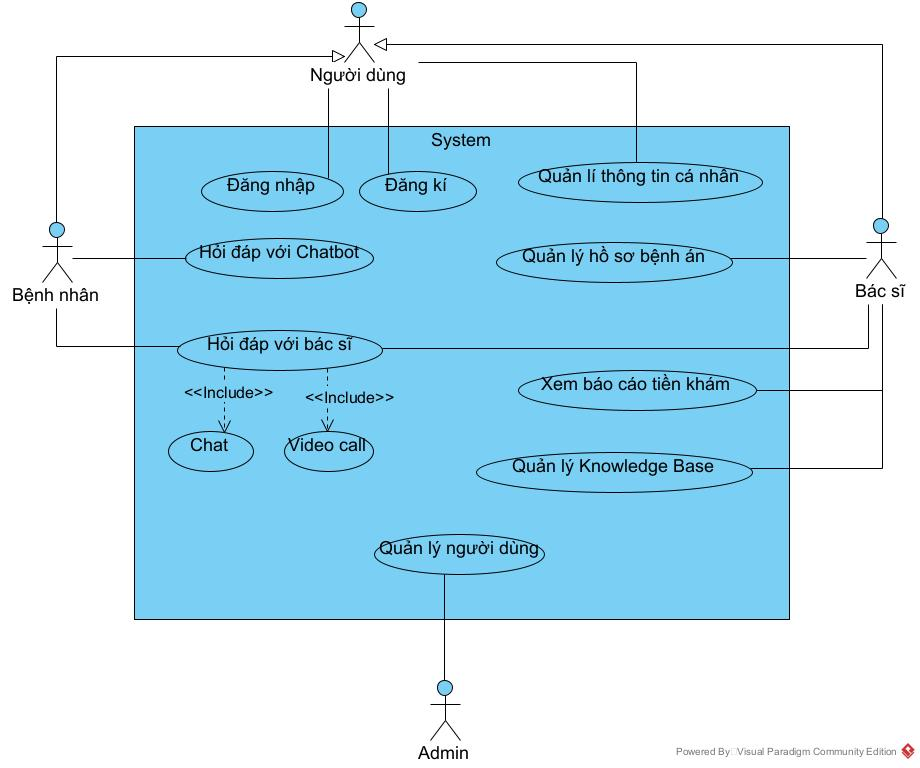
\includegraphics[width=0.95\linewidth,height=0.7\textheight,keepaspectratio]{chuong5/hinh/usecase_tong_quan.jpg}
  \caption{Sơ đồ usecase tổng quan của hệ thống}
\end{figure}

\subsection{Usecase Đăng ký (Sign Up)}
\begin{itemize}
  \item Cho phép người dùng mới tạo tài khoản trên hệ thống với vai trò tương ứng (bệnh nhân hoặc bác sĩ).
\end{itemize}

\subsection{Usecase Đăng nhập (Sign In)}
\begin{itemize}
  \item Xác thực danh tính người dùng để truy cập vào các chức năng tương ứng với quyền hạn của mình.
\end{itemize}

\subsection{Usecase Quản lý thông tin cá nhân (Profile Management)}
\begin{itemize}
  \item Cho phép xem, cập nhật và chỉnh sửa thông tin cá nhân, liên hệ, chuyên môn (đối với bác sĩ) hoặc thông tin cơ bản (đối với bệnh nhân).
\end{itemize}

\subsection{Usecase Hỏi đáp với Chatbot}
\begin{itemize}
  \item Bệnh nhân gửi mô tả triệu chứng và hình ảnh tổn thương da để nhận kết quả tiền chẩn đoán, giải thích ngắn gọn, dễ hiểu.
  \item Hệ thống tự động trích xuất các dữ kiện lâm sàng (\textit{clinical facts}) và tra cứu cơ sở tri thức (Knowledge Base - KB), ca bệnh tương tự để phục vụ tư vấn hoặc chuyển tiếp cho bác sĩ.
\end{itemize}

\subsection{Usecase Hỏi đáp với bác sĩ}
\begin{itemize}
  \item Cho phép bệnh nhân kết nối, tư vấn trực tiếp với bác sĩ khi cần thăm khám chuyên sâu. Gồm 2 chức năng thành phần:
  \begin{itemize}
    \item \textbf{Chat}: Nhắn tin trao đổi trực tiếp văn bản, hình ảnh.
    \item \textbf{Video call}: Thực hiện cuộc gọi video trực tuyến để bác sĩ quan sát rõ hơn tình trạng bệnh.
  \end{itemize}
  \item \textit{Lưu ý}: Trong khi chờ bác sĩ tiếp nhận, bệnh nhân tương tác với chatbot; nội dung này sẽ được tổng hợp lại cho bác sĩ trước khi trao đổi trực tiếp với bệnh nhân
\end{itemize}

\subsection{Usecase Xem báo cáo tiền khám}
\begin{itemize}
  \item Bác sĩ xem báo cáo tổng hợp tự động về bệnh nhân:
  \begin{itemize}
    \item Dựa trên các dữ kiện lâm sàng (\textit{clinical facts}) thu thập từ cuộc chat của bệnh nhân với chatbot.
    \item Hiển thị căn cứ/nguồn lập luận từ KB, biểu đồ tri thức (\textit{Knowledge Graph}) trực quan và lịch sử bệnh án liên quan.
  \end{itemize}
\end{itemize}

\subsection{Usecase Quản lý hồ sơ bệnh án}
\begin{itemize}
  \item Bác sĩ xem chi tiết hồ sơ bệnh nhân, lịch sử các lần khám.
  \item Bác sĩ cập nhật, chỉnh sửa kết luận chẩn đoán sau mỗi lượt khám; lưu trữ ca bệnh và hình ảnh làm chuẩn dữ liệu phục vụ tái huấn luyện mô hình đa CNN (\textit{multi-CNN}).
\end{itemize}

\subsection{Usecase Quản lý Knowledge Base (KB)}
\begin{itemize}
  \item Bác sĩ tải lên tài liệu y khoa, giáo trình chuyên ngành để làm giàu tri thức hệ thống.
  \item Tra cứu, kiểm duyệt và phối hợp cùng mô hình/chatbot để chuẩn hóa, mở rộng cơ sở tri thức da liễu phục vụ RAG.
\end{itemize}

\subsection{Quản lý người dùng}
\begin{itemize}
  \item Admin kiểm tra hồ sơ bác sĩ trước khi duyệt
\end{itemize}

\section{Thiết kế cơ sở dữ liệu}

\subsection{Thiết kế class}
\begin{figure}[H]
  \centering
  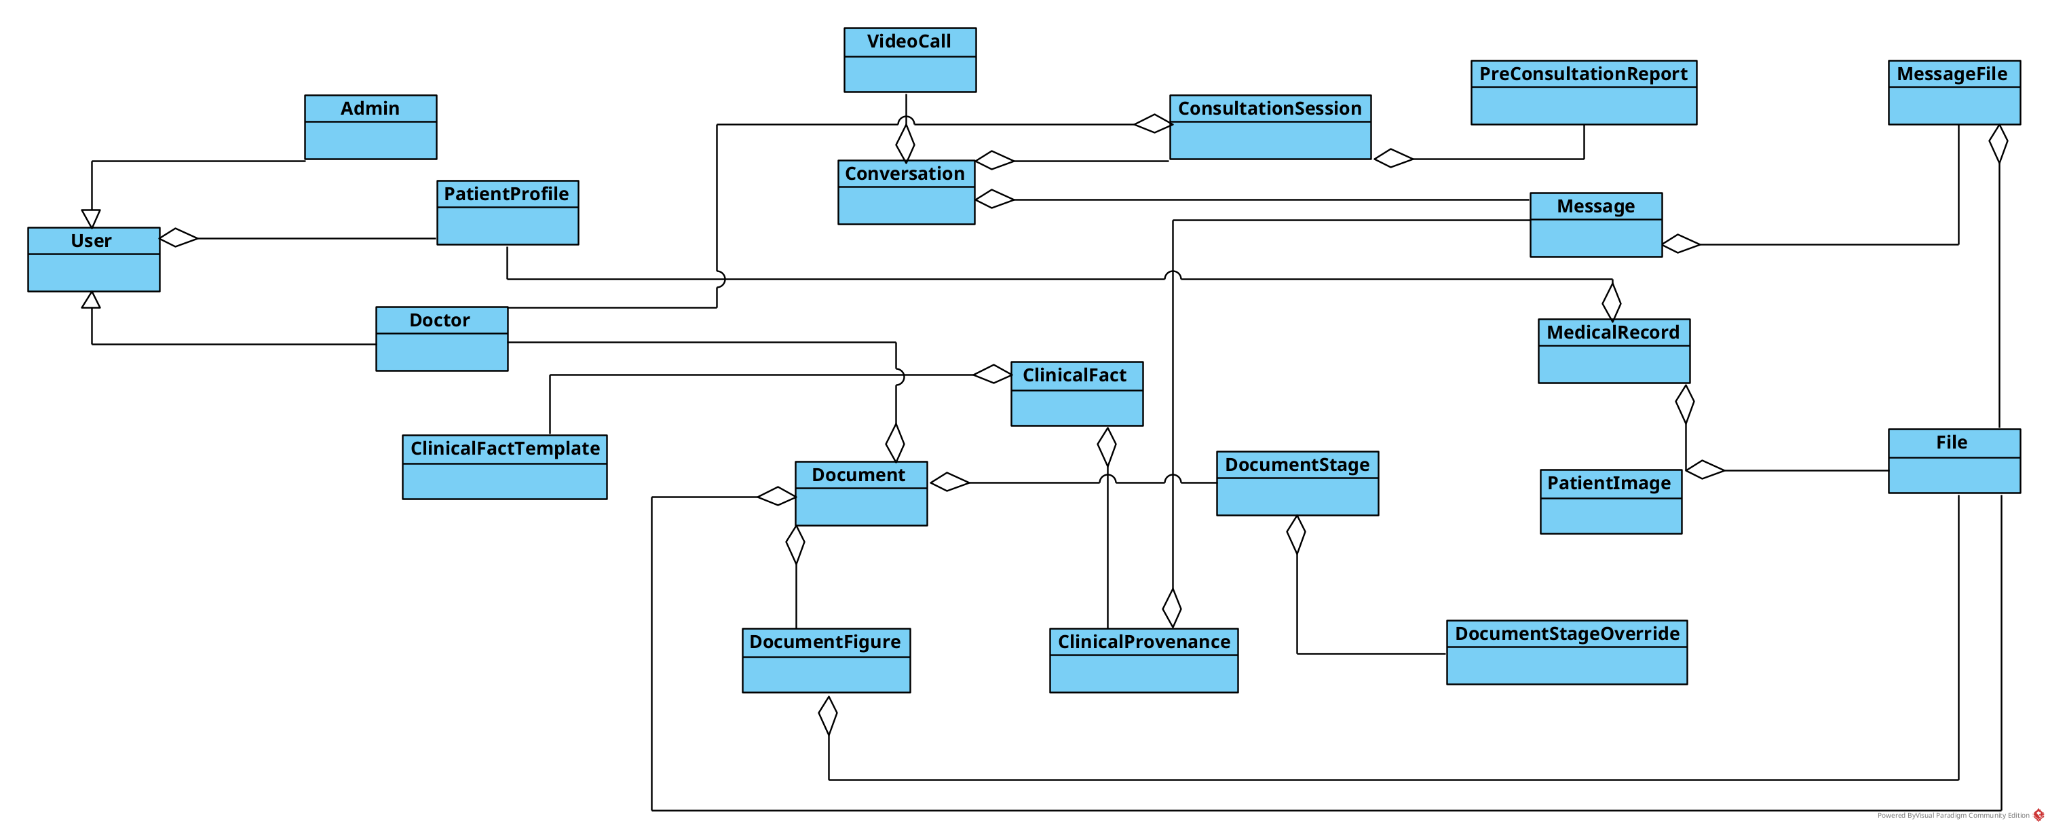
\includegraphics[width=0.95\linewidth,height=0.7\textheight,keepaspectratio]{chuong5/hinh/so_do_lop.png}
  \caption{Sơ đồ lớp của hệ thống}
\end{figure}

\subsection{Thiết kế CSDL}
\begin{figure}[H]
  \centering
  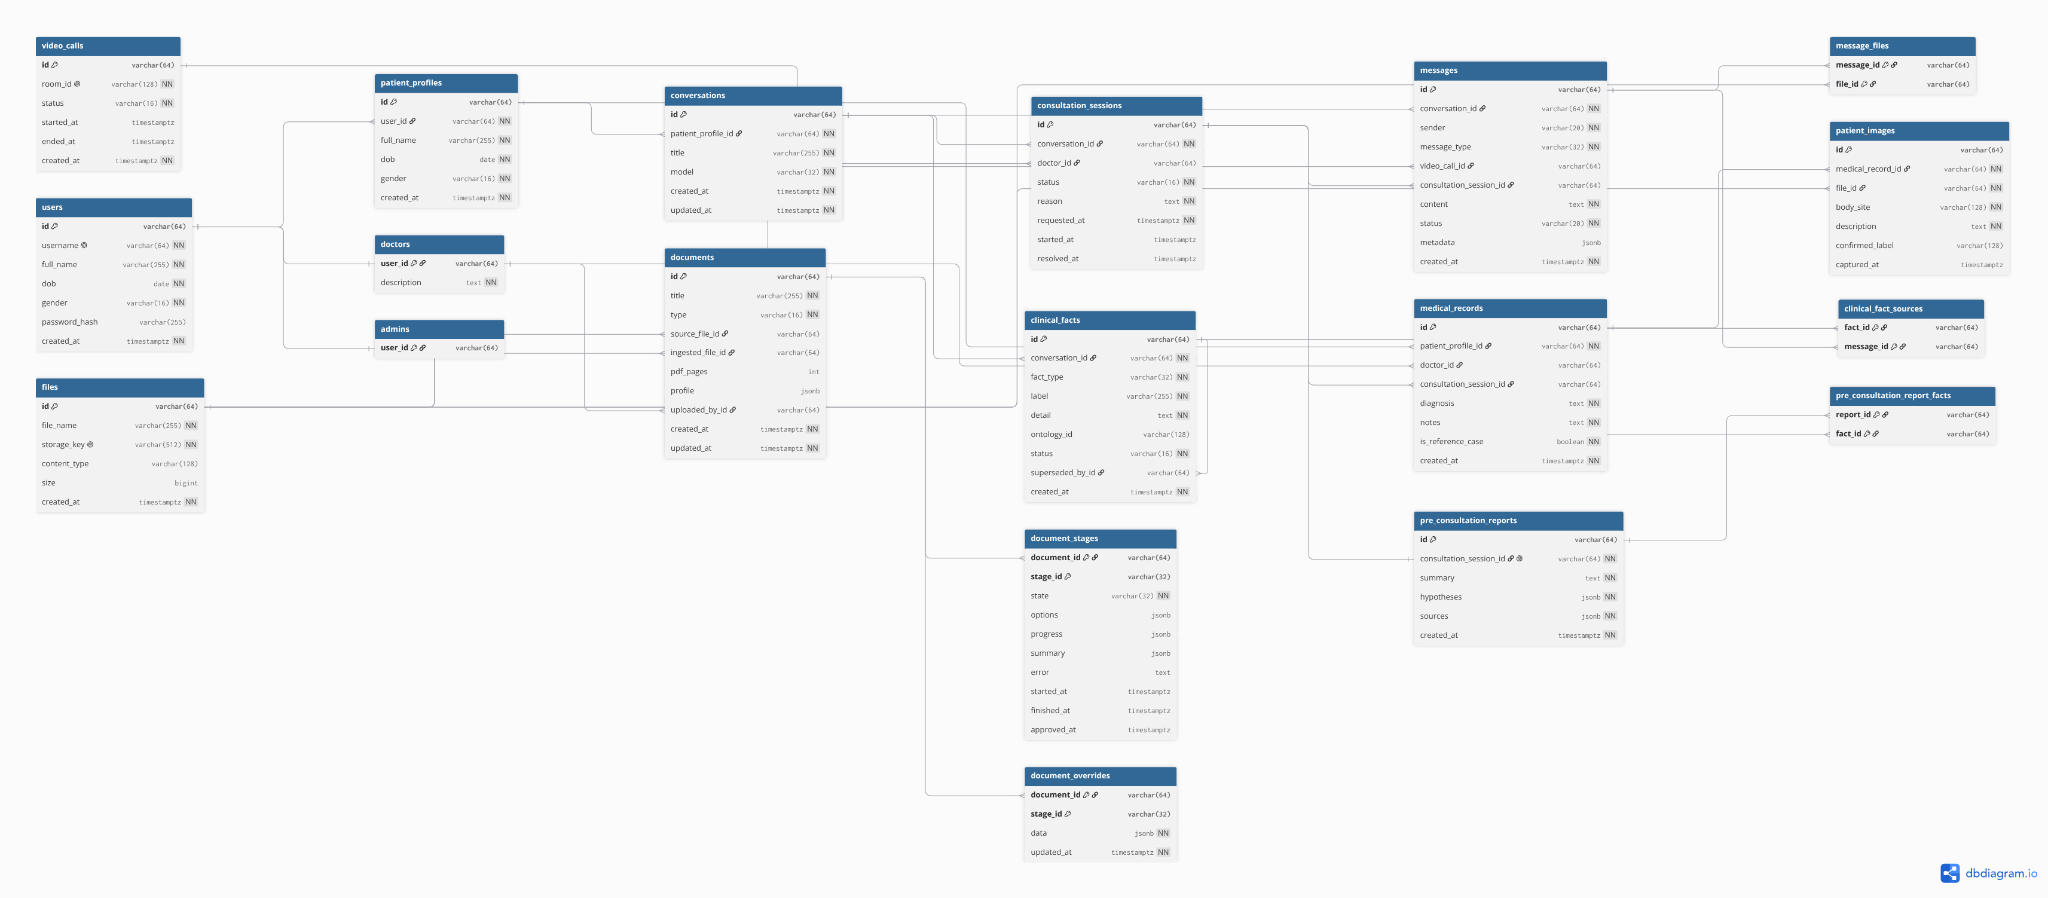
\includegraphics[width=0.95\linewidth,height=0.7\textheight,keepaspectratio]{chuong5/hinh/so_do_csdl.png}
  \caption{Sơ đồ cơ sở dữ liệu của hệ thống}
\end{figure}

\paragraph{Nhóm Người dùng}

\subparagraph{users -- tài khoản}

Field chung của mọi loại tài khoản. Vai trò bác sĩ / quản trị là bảng con 1-1 (doctors, admins), bệnh nhân là patient\_profiles. Chưa có API đăng ký / đăng nhập.
\begin{longtable}{|>{\raggedright\arraybackslash}p{0.250\dimexpr\linewidth-8\tabcolsep\relax}|>{\raggedright\arraybackslash}p{0.250\dimexpr\linewidth-8\tabcolsep\relax}|>{\raggedright\arraybackslash}p{0.250\dimexpr\linewidth-8\tabcolsep\relax}|>{\raggedright\arraybackslash}p{0.250\dimexpr\linewidth-8\tabcolsep\relax}|}
\hline
\textbf{Field} & \textbf{Kiểu} & \textbf{Null} & \textbf{Ý nghĩa} \\ \hline
\endhead
id & varchar(64) PK & không & Mã tài khoản, DB sinh. \\ \hline
username & varchar(64) & không, unique & Tên đăng nhập. \\ \hline
full\_name & varchar(255) & không & Họ tên đầy đủ. \\ \hline
dob & date & không & Ngày sinh. \\ \hline
gender & varchar(16) & không & male | female. \\ \hline
password\_hash & varchar(255) & có & Hash mật khẩu. NULL = tài khoản mẫu chưa đặt mật khẩu, chưa đăng nhập được. \\ \hline
created\_at & timestamptz & không & Thời điểm tạo tài khoản. \\ \hline
\end{longtable}

\subparagraph{patient\_profiles -- hồ sơ bệnh nhân}

Một tài khoản quản lý được nhiều hồ sơ (bản thân, người nhà). Hội thoại, bệnh án và dữ kiện lâm sàng đều gắn vào hồ sơ này, không gắn thẳng vào users.
\begin{longtable}{|>{\raggedright\arraybackslash}p{0.227\dimexpr\linewidth-8\tabcolsep\relax}|>{\raggedright\arraybackslash}p{0.273\dimexpr\linewidth-8\tabcolsep\relax}|>{\raggedright\arraybackslash}p{0.250\dimexpr\linewidth-8\tabcolsep\relax}|>{\raggedright\arraybackslash}p{0.250\dimexpr\linewidth-8\tabcolsep\relax}|}
\hline
\textbf{Field} & \textbf{Kiểu} & \textbf{Null} & \textbf{Ý nghĩa} \\ \hline
\endhead
id & varchar(64) PK & không & Mã hồ sơ. \\ \hline
user\_id & varchar(64) FK → users.id & không & Tài khoản quản lý hồ sơ. ON DELETE CASCADE. Có index. \\ \hline
full\_name & varchar(255) & không & Họ tên người bệnh (có thể khác chủ tài khoản). \\ \hline
dob & date & không & Ngày sinh người bệnh. \\ \hline
gender & varchar(16) & không & male | female. \\ \hline
created\_at & timestamptz & không & Thời điểm tạo hồ sơ. \\ \hline
\end{longtable}

\subparagraph{doctors -- vai trò bác sĩ}

Quan hệ 1-1 với users: PK đồng thời là FK nên một user chỉ có tối đa một dòng bác sĩ. Các bảng khác trỏ vào doctors.user\_id (không phải users.id) để DB chặn việc gán người không phải bác sĩ.
\begin{longtable}{|>{\raggedright\arraybackslash}p{0.250\dimexpr\linewidth-8\tabcolsep\relax}|>{\raggedright\arraybackslash}p{0.250\dimexpr\linewidth-8\tabcolsep\relax}|>{\raggedright\arraybackslash}p{0.250\dimexpr\linewidth-8\tabcolsep\relax}|>{\raggedright\arraybackslash}p{0.250\dimexpr\linewidth-8\tabcolsep\relax}|}
\hline
\textbf{Field} & \textbf{Kiểu} & \textbf{Null} & \textbf{Ý nghĩa} \\ \hline
\endhead
user\_id & varchar(64) PK, FK → users.id & không & Tài khoản được cấp vai trò bác sĩ. ON DELETE CASCADE. \\ \hline
description & text & không & Giới thiệu chuyên môn của bác sĩ. \\ \hline
\end{longtable}

\subparagraph{admins -- vai trò quản trị}

Quan hệ 1-1 với users, đánh dấu tài khoản quản trị (khu /admin/documents). Chưa có field riêng.
\begin{longtable}{|>{\raggedright\arraybackslash}p{0.250\dimexpr\linewidth-8\tabcolsep\relax}|>{\raggedright\arraybackslash}p{0.250\dimexpr\linewidth-8\tabcolsep\relax}|>{\raggedright\arraybackslash}p{0.250\dimexpr\linewidth-8\tabcolsep\relax}|>{\raggedright\arraybackslash}p{0.250\dimexpr\linewidth-8\tabcolsep\relax}|}
\hline
\textbf{Field} & \textbf{Kiểu} & \textbf{Null} & \textbf{Ý nghĩa} \\ \hline
\endhead
user\_id & varchar(64) PK, FK → users.id & không & Tài khoản quản trị. ON DELETE CASCADE. \\ \hline
\end{longtable}

\paragraph{Nhóm Hội thoại \& tư vấn}

\subparagraph{conversations -- cuộc hội thoại}

Một cuộc chat của một hồ sơ bệnh nhân. Chủ tài khoản suy ra qua patient\_profiles.user\_id, không lưu lặp ở đây.
\begin{longtable}{|>{\raggedright\arraybackslash}p{0.250\dimexpr\linewidth-8\tabcolsep\relax}|>{\raggedright\arraybackslash}p{0.228\dimexpr\linewidth-8\tabcolsep\relax}|>{\raggedright\arraybackslash}p{0.272\dimexpr\linewidth-8\tabcolsep\relax}|>{\raggedright\arraybackslash}p{0.250\dimexpr\linewidth-8\tabcolsep\relax}|}
\hline
\textbf{Field} & \textbf{Kiểu} & \textbf{Null} & \textbf{Ý nghĩa} \\ \hline
\endhead
id & varchar(64) PK & không & Mã hội thoại. \\ \hline
patient\_profile\_id & varchar(64) FK → patient\_profiles.id & không & Hồ sơ bệnh nhân sở hữu hội thoại. \\ \hline
title & varchar(255) & không, mặc định & Tiêu đề hiển thị trong danh sách chat. \\ \hline
model & varchar(32) & không & Id ngắn của model trong AGENT\_MODEL\_CHOICES (không phải chuỗi provider:model); worker tự map sang model thật khi chạy lượt, nên đổi danh sách model không cần migration. \\ \hline
created\_at & timestamptz & không & Thời điểm tạo. \\ \hline
updated\_at & timestamptz & không & Lần cập nhật gần nhất (tự cập nhật khi sửa). \\ \hline
\end{longtable}

\subparagraph{messages -- tin nhắn}

Một luồng chung cho AI, bệnh nhân và bác sĩ, phân biệt bằng sender. Các mốc tư vấn và cuộc gọi video cũng hiện thành tin trong luồng này.
\begin{longtable}{|>{\raggedright\arraybackslash}p{0.214\dimexpr\linewidth-8\tabcolsep\relax}|>{\raggedright\arraybackslash}p{0.230\dimexpr\linewidth-8\tabcolsep\relax}|>{\raggedright\arraybackslash}p{0.220\dimexpr\linewidth-8\tabcolsep\relax}|>{\raggedright\arraybackslash}p{0.336\dimexpr\linewidth-8\tabcolsep\relax}|}
\hline
\textbf{Field} & \textbf{Kiểu} & \textbf{Null} & \textbf{Ý nghĩa} \\ \hline
\endhead
id & varchar(64) PK & không & Mã tin nhắn. \\ \hline
conversation\_id & varchar(64) FK → conversations.id & không & Hội thoại chứa tin. \\ \hline
sender & varchar(20) & không & Người gửi: patient | ai | doctor. \\ \hline
message\_type & varchar(32) & không, mặc định text & Loại tin: text, attached (có đính kèm), video\_call, consultation\_requested, consultation\_accepted, consultation\_resolved. Là cột riêng để lọc / đếm theo loại. \\ \hline
video\_call\_id & varchar(64) FK → video\_calls.id & có & Chỉ điền với message\_type = video\_call. ON DELETE SET NULL. \\ \hline
consultation\_session\_id & varchar(64) FK → consultation\_sessions.id & có & Chỉ điền với 3 tin mốc consultation\_*: tin thuộc phiên tư vấn nào. ON DELETE SET NULL. Có index. \\ \hline
content & text & không, mặc định '' & Nội dung chữ. \\ \hline
status & varchar(20) & không & Trạng thái xử lý: queued | done | question (còn khai báo pending | streaming). question = agent đang chờ người dùng trả lời. \\ \hline
metadata & jsonb & có & Dữ liệu phụ (ORM đặt tên attribute là extra vì metadata trùng tên reserved của SQLAlchemy). Tin AI: reasoning[] (các bước lập luận), choice (câu hỏi lại), sources[] (nguồn trích dẫn). Tin người dùng: attached\_files, is\_option\_response. \\ \hline
created\_at & timestamptz & không & Thời điểm tạo tin. \\ \hline
\end{longtable}

\subparagraph{message\_files -- tệp đính kèm của tin nhắn (n-n)}

Bảng nối giữa tin nhắn và file. Một tin có thể đính kèm nhiều file, một file có thể được dùng lại ở nhiều chỗ.
\begin{longtable}{|>{\raggedright\arraybackslash}p{0.250\dimexpr\linewidth-8\tabcolsep\relax}|>{\raggedright\arraybackslash}p{0.250\dimexpr\linewidth-8\tabcolsep\relax}|>{\raggedright\arraybackslash}p{0.250\dimexpr\linewidth-8\tabcolsep\relax}|>{\raggedright\arraybackslash}p{0.250\dimexpr\linewidth-8\tabcolsep\relax}|}
\hline
\textbf{Field} & \textbf{Kiểu} & \textbf{Null} & \textbf{Ý nghĩa} \\ \hline
\endhead
message\_id & varchar(64) PK, FK → messages.id & không & Tin nhắn. ON DELETE CASCADE. \\ \hline
file\_id & varchar(64) PK, FK → files.id & không & File đính kèm. ON DELETE CASCADE. \\ \hline
\end{longtable}

\subparagraph{consultation\_sessions -- phiên tư vấn bác sĩ}

Mốc đánh dấu một lần bệnh nhân nhờ bác sĩ hỗ trợ; bảng này không chứa tin nhắn. Tin trao đổi nằm trong messages (sender = doctor), ba mốc yêu cầu / nhận / đóng là tin consultation\_* trỏ về phiên. Bác sĩ xem luồng chat từ đầu đến tin consultation\_resolved của phiên (phiên còn mở: tới hiện tại). Bệnh nhân vẫn chat AI song song. Mới có schema.
\begin{longtable}{|>{\raggedright\arraybackslash}p{0.250\dimexpr\linewidth-8\tabcolsep\relax}|>{\raggedright\arraybackslash}p{0.250\dimexpr\linewidth-8\tabcolsep\relax}|>{\raggedright\arraybackslash}p{0.250\dimexpr\linewidth-8\tabcolsep\relax}|>{\raggedright\arraybackslash}p{0.250\dimexpr\linewidth-8\tabcolsep\relax}|}
\hline
\textbf{Field} & \textbf{Kiểu} & \textbf{Null} & \textbf{Ý nghĩa} \\ \hline
\endhead
id & varchar(64) PK & không & Mã phiên. \\ \hline
conversation\_id & varchar(64) FK → conversations.id & không & Hội thoại có phiên tư vấn. ON DELETE CASCADE. Có index. \\ \hline
doctor\_id & varchar(64) FK → doctors.user\_id & có & Bác sĩ nhận ca. NULL khi chưa ai nhận. ON DELETE SET NULL. \\ \hline
status & varchar(16) & không, mặc định pending & pending (chờ bác sĩ nhận) → active (đang trao đổi) → resolved (đã đóng). \\ \hline
reason & text & không & Lý do bệnh nhân nhờ bác sĩ. \\ \hline
requested\_at & timestamptz & không & Lúc bệnh nhân gửi yêu cầu. \\ \hline
started\_at & timestamptz & có & Lúc bác sĩ nhận. \\ \hline
resolved\_at & timestamptz & có & Lúc đóng phiên. \\ \hline
\end{longtable}

Ràng buộc:
\begin{itemize}
  \item CHECK doctor\_when\_not\_pending: status = 'pending' OR doctor\_id IS NOT NULL --- phiên đã nhận hoặc đã đóng thì bắt buộc có bác sĩ.
  \item CHECK resolved\_at\_when\_resolved: status <> 'resolved' OR resolved\_at IS NOT NULL.
  \item Unique một phần uq\_consultation\_sessions\_open\_per\_conversation trên conversation\_id với điều kiện status <> 'resolved' --- mỗi hội thoại tối đa 1 phiên đang mở, vì tin bác sĩ gắn với phiên theo khoảng thời gian, hai phiên mở cùng lúc sẽ không phân biệt được.
\end{itemize}

\subparagraph{video\_calls -- cuộc gọi video}

Tách bảng riêng (không chỉ nằm trong messages.metadata) vì cuộc gọi có vòng đời pending → ongoing → ended được cập nhật sau khi tin nhắn đã tạo. Tin message\_type = video\_call trỏ tới đây qua messages.video\_call\_id. Mới có schema.
\begin{longtable}{|>{\raggedright\arraybackslash}p{0.250\dimexpr\linewidth-8\tabcolsep\relax}|>{\raggedright\arraybackslash}p{0.250\dimexpr\linewidth-8\tabcolsep\relax}|>{\raggedright\arraybackslash}p{0.250\dimexpr\linewidth-8\tabcolsep\relax}|>{\raggedright\arraybackslash}p{0.250\dimexpr\linewidth-8\tabcolsep\relax}|}
\hline
\textbf{Field} & \textbf{Kiểu} & \textbf{Null} & \textbf{Ý nghĩa} \\ \hline
\endhead
id & varchar(64) PK & không & Mã cuộc gọi. \\ \hline
room\_id & varchar(128) & không, unique & Mã phòng video. \\ \hline
status & varchar(16) & không, mặc định pending & pending | ongoing | ended. \\ \hline
started\_at & timestamptz & có & Lúc bắt đầu gọi. \\ \hline
ended\_at & timestamptz & có & Lúc kết thúc. \\ \hline
created\_at & timestamptz & không & Lúc tạo cuộc gọi. \\ \hline
\end{longtable}

\paragraph{Nhóm Bệnh án}

\subparagraph{medical\_records -- bệnh án}

Bệnh án do bác sĩ ghi cho một hồ sơ bệnh nhân; một hồ sơ có nhiều bệnh án. Không gắn với phiên tư vấn cụ thể. Mới có schema.
\begin{longtable}{|>{\raggedright\arraybackslash}p{0.250\dimexpr\linewidth-8\tabcolsep\relax}|>{\raggedright\arraybackslash}p{0.250\dimexpr\linewidth-8\tabcolsep\relax}|>{\raggedright\arraybackslash}p{0.250\dimexpr\linewidth-8\tabcolsep\relax}|>{\raggedright\arraybackslash}p{0.250\dimexpr\linewidth-8\tabcolsep\relax}|}
\hline
\textbf{Field} & \textbf{Kiểu} & \textbf{Null} & \textbf{Ý nghĩa} \\ \hline
\endhead
id & varchar(64) PK & không & Mã bệnh án. \\ \hline
patient\_profile\_id & varchar(64) FK → patient\_profiles.id & không & Hồ sơ bệnh nhân. ON DELETE CASCADE. Có index. \\ \hline
doctor\_id & varchar(64) FK → doctors.user\_id & có & Bác sĩ ghi bệnh án. ON DELETE SET NULL --- bác sĩ bị xoá thì bệnh án vẫn giữ. \\ \hline
diagnosis & text & không & Chẩn đoán của bác sĩ. \\ \hline
notes & text & không, mặc định '' & Ghi chú thêm. \\ \hline
is\_reference\_case & boolean & không, mặc định false & Ca bệnh tham khảo: bác sĩ xác nhận dùng làm dữ liệu cho KB / chatbot tra ca tương tự (phải ẩn định danh khi đưa vào KB). \\ \hline
created\_at & timestamptz & không & Lúc ghi bệnh án. \\ \hline
\end{longtable}

\subparagraph{patient\_images -- ảnh bệnh}

Ảnh bệnh do bác sĩ gắn vào bệnh án. Trỏ FK tới files thay vì chép file, nên bác sĩ chọn lại được ảnh bệnh nhân đã gửi trong chat mà không tạo bản sao trong MinIO. Mới có schema.
\begin{longtable}{|>{\raggedright\arraybackslash}p{0.250\dimexpr\linewidth-8\tabcolsep\relax}|>{\raggedright\arraybackslash}p{0.250\dimexpr\linewidth-8\tabcolsep\relax}|>{\raggedright\arraybackslash}p{0.250\dimexpr\linewidth-8\tabcolsep\relax}|>{\raggedright\arraybackslash}p{0.250\dimexpr\linewidth-8\tabcolsep\relax}|}
\hline
\textbf{Field} & \textbf{Kiểu} & \textbf{Null} & \textbf{Ý nghĩa} \\ \hline
\endhead
id & varchar(64) PK & không & Mã ảnh. \\ \hline
medical\_record\_id & varchar(64) FK → medical\_records.id & không & Bệnh án chứa ảnh. ON DELETE CASCADE. Có index. \\ \hline
file\_id & varchar(64) FK → files.id & không & File ảnh trong MinIO. ON DELETE CASCADE. \\ \hline
body\_site & varchar(128) & không, mặc định '' & Vị trí trên cơ thể. \\ \hline
description & text & không, mặc định '' & Mô tả tổn thương. \\ \hline
confirmed\_label & varchar(128) & có & Nhãn bác sĩ xác nhận, nên khớp tên lớp của CNN để dùng làm dữ liệu huấn luyện. \\ \hline
captured\_at & timestamptz & có & Thời điểm chụp ảnh. \\ \hline
\end{longtable}

\paragraph{Nhóm Lâm sàng}

Luồng ý tưởng: agent trích dữ kiện lâm sàng từ hội thoại, mỗi dữ kiện luôn tạo từ một mẫu chuẩn, ghi lại tin nhắn nguồn, và khi bệnh nhân nhờ bác sĩ thì có một báo cáo tóm tắt cho phiên đó. Cả nhóm mới có schema, chưa có bước trích xuất.

\subparagraph{clinical\_fact\_templates -- mẫu dữ kiện lâm sàng}

Danh mục chuẩn (ví dụ "ngứa", "dị ứng penicillin"). Agent chỉ được trích fact theo mẫu có sẵn để nhãn và ontology\_id nhất quán giữa các bệnh nhân.
\begin{longtable}{|>{\raggedright\arraybackslash}p{0.250\dimexpr\linewidth-8\tabcolsep\relax}|>{\raggedright\arraybackslash}p{0.250\dimexpr\linewidth-8\tabcolsep\relax}|>{\raggedright\arraybackslash}p{0.250\dimexpr\linewidth-8\tabcolsep\relax}|>{\raggedright\arraybackslash}p{0.250\dimexpr\linewidth-8\tabcolsep\relax}|}
\hline
\textbf{Field} & \textbf{Kiểu} & \textbf{Null} & \textbf{Ý nghĩa} \\ \hline
\endhead
id & varchar(64) PK & không & Mã mẫu. \\ \hline
fact\_type & varchar(32) & không & Loại: symptom (triệu chứng cơ năng), lesion (tổn thương da), history (tiền sử / diễn tiến), medication (thuốc), allergy (dị ứng), image\_finding (kết quả phân loại ảnh, chỉ là giả thuyết), other. \\ \hline
label & varchar(255) & không, unique & Tên chuẩn của mẫu. \\ \hline
description & text & không, mặc định '' & Gợi ý cho agent / bác sĩ biết cần hỏi và ghi gì vào clinical\_facts.detail. \\ \hline
ontology\_id & varchar(128) & có & Id DermO / PrimeKG đã chuẩn hoá, dùng để vẽ KG liên quan bệnh nhân. \\ \hline
\end{longtable}

\subparagraph{clinical\_facts -- dữ kiện lâm sàng}

Dữ kiện của hồ sơ bệnh nhân (không thuộc riêng một cuộc chat), luôn tạo từ một mẫu. Không sửa đè: bệnh nhân đính chính thì tạo fact mới và đánh dấu fact cũ superseded, để bác sĩ vẫn thấy lịch sử khai báo. Hội thoại sinh ra fact truy ngược qua clinical\_provenances → messages.
\begin{longtable}{|>{\raggedright\arraybackslash}p{0.250\dimexpr\linewidth-8\tabcolsep\relax}|>{\raggedright\arraybackslash}p{0.250\dimexpr\linewidth-8\tabcolsep\relax}|>{\raggedright\arraybackslash}p{0.250\dimexpr\linewidth-8\tabcolsep\relax}|>{\raggedright\arraybackslash}p{0.250\dimexpr\linewidth-8\tabcolsep\relax}|}
\hline
\textbf{Field} & \textbf{Kiểu} & \textbf{Null} & \textbf{Ý nghĩa} \\ \hline
\endhead
id & varchar(64) PK & không & Mã fact. \\ \hline
patient\_profile\_id & varchar(64) FK → patient\_profiles.id & không & Hồ sơ bệnh nhân sở hữu fact. ON DELETE CASCADE. Có index. \\ \hline
template\_id & varchar(64) FK → clinical\_fact\_templates.id & không & Mẫu của fact; loại / nhãn / ontology lấy từ mẫu. ON DELETE RESTRICT --- không xoá được mẫu đang có fact dùng. Có index. \\ \hline
detail & text & không, mặc định '' & Giá trị cụ thể của bệnh nhân: vị trí, thời gian khởi phát, mức độ, diễn tiến... \\ \hline
status & varchar(16) & không, mặc định active & active | superseded (đã bị fact mới thay). \\ \hline
superseded\_by\_id & varchar(64) FK → clinical\_facts.id (tự tham chiếu) & có & Fact mới thay thế fact này. ON DELETE SET NULL. \\ \hline
created\_at & timestamptz & không & Lúc ghi fact. \\ \hline
\end{longtable}

\subparagraph{clinical\_provenances -- nguồn gốc của fact (n-n)}

Bảng nối giữa fact và tin nhắn, thể hiện entity ClinicalProvenance. Một fact có

thể đến từ nhiều tin (kể cả ở nhiều hội thoại), một tin có thể sinh nhiều fact. Fact do bác sĩ tự nhập thì không có dòng nào ở đây. Sau này muốn thêm thông tin riêng cho mỗi cặp (đoạn trích, độ tin cậy) thì thêm cột vào bảng này.
\begin{longtable}{|>{\raggedright\arraybackslash}p{0.250\dimexpr\linewidth-8\tabcolsep\relax}|>{\raggedright\arraybackslash}p{0.250\dimexpr\linewidth-8\tabcolsep\relax}|>{\raggedright\arraybackslash}p{0.250\dimexpr\linewidth-8\tabcolsep\relax}|>{\raggedright\arraybackslash}p{0.250\dimexpr\linewidth-8\tabcolsep\relax}|}
\hline
\textbf{Field} & \textbf{Kiểu} & \textbf{Null} & \textbf{Ý nghĩa} \\ \hline
\endhead
fact\_id & varchar(64) PK, FK → clinical\_facts.id & không & Fact. ON DELETE CASCADE. \\ \hline
message\_id & varchar(64) PK, FK → messages.id & không & Tin nhắn gốc làm bằng chứng. ON DELETE CASCADE. \\ \hline
\end{longtable}

\subparagraph{pre\_consultation\_reports -- báo cáo tiền tư vấn}

Báo cáo AI tóm tắt cho bác sĩ đọc trước khi nhận ca, 1 báo cáo / phiên tư vấn. Chỉ là gợi ý hỗ trợ, không phải chẩn đoán y khoa. Tạm thời chỉ có phần tóm tắt; fact lâm sàng bác sĩ xem trực tiếp từ hồ sơ bệnh nhân.
\begin{longtable}{|>{\raggedright\arraybackslash}p{0.250\dimexpr\linewidth-8\tabcolsep\relax}|>{\raggedright\arraybackslash}p{0.250\dimexpr\linewidth-8\tabcolsep\relax}|>{\raggedright\arraybackslash}p{0.250\dimexpr\linewidth-8\tabcolsep\relax}|>{\raggedright\arraybackslash}p{0.250\dimexpr\linewidth-8\tabcolsep\relax}|}
\hline
\textbf{Field} & \textbf{Kiểu} & \textbf{Null} & \textbf{Ý nghĩa} \\ \hline
\endhead
id & varchar(64) PK & không & Mã báo cáo. \\ \hline
consultation\_session\_id & varchar(64) FK → consultation\_sessions.id & không, unique & Phiên tư vấn của báo cáo; unique tạo quan hệ 1-1. ON DELETE CASCADE. \\ \hline
summary & text & không & Nội dung tóm tắt. \\ \hline
created\_at & timestamptz & không & Lúc sinh báo cáo. \\ \hline
\end{longtable}

\paragraph{Nhóm File}

\subparagraph{files -- metadata file trong MinIO}

Dùng chung cho ảnh đính kèm tin nhắn, ảnh bệnh trong bệnh án và file của tài liệu. Nội dung file nằm ở MinIO, không nằm trong DB.
\begin{longtable}{|>{\raggedright\arraybackslash}p{0.250\dimexpr\linewidth-8\tabcolsep\relax}|>{\raggedright\arraybackslash}p{0.250\dimexpr\linewidth-8\tabcolsep\relax}|>{\raggedright\arraybackslash}p{0.250\dimexpr\linewidth-8\tabcolsep\relax}|>{\raggedright\arraybackslash}p{0.250\dimexpr\linewidth-8\tabcolsep\relax}|}
\hline
\textbf{Field} & \textbf{Kiểu} & \textbf{Null} & \textbf{Ý nghĩa} \\ \hline
\endhead
id & varchar(64) PK & không & Mã file. \\ \hline
file\_name & varchar(255) & không & Tên hiển thị (ví dụ tên file gốc người dùng upload). \\ \hline
storage\_key & varchar(512) & không, unique & Khoá đầy đủ của object trong bucket MinIO (không phải đường dẫn tương đối trong thư mục của entity). \\ \hline
content\_type & varchar(128) & có & MIME type, ví dụ application/pdf. \\ \hline
size & bigint & có & Dung lượng, đơn vị byte. \\ \hline
created\_at & timestamptz & không & Lúc tạo bản ghi. \\ \hline
\end{longtable}

\paragraph{Nhóm Tài liệu (pipeline số hoá sách)}

Admin upload PDF → qua 4 bước (ingest → toc → chunks → index), mỗi bước người duyệt phải approve trước khi bước sau chạy. Entity lồng nhau: Document → DocumentStage → DocumentStageOverride.

\subparagraph{documents -- tài liệu}
\begin{longtable}{|>{\raggedright\arraybackslash}p{0.250\dimexpr\linewidth-8\tabcolsep\relax}|>{\raggedright\arraybackslash}p{0.250\dimexpr\linewidth-8\tabcolsep\relax}|>{\raggedright\arraybackslash}p{0.250\dimexpr\linewidth-8\tabcolsep\relax}|>{\raggedright\arraybackslash}p{0.250\dimexpr\linewidth-8\tabcolsep\relax}|}
\hline
\textbf{Field} & \textbf{Kiểu} & \textbf{Null} & \textbf{Ý nghĩa} \\ \hline
\endhead
id & varchar(64) PK & không & Mã tài liệu; cũng là tên thư mục document/<id>/ trong MinIO và document\_id trong payload Qdrant. \\ \hline
title & varchar(255) & không & Tiêu đề. \\ \hline
type & varchar(16) & không, mặc định book & book | image | video | other. Hiện chỉ book đi qua pipeline. \\ \hline
source\_file\_id & varchar(64) FK → files.id & có & File gốc người dùng upload (source.pdf). ON DELETE SET NULL. \\ \hline
ingested\_file\_id & varchar(64) FK → files.id & có & Kết quả bước ingest (pages.jsonl); chỉ có khi đã qua bước ingest. ON DELETE SET NULL. \\ \hline
pdf\_pages & int & có & Số trang PDF; chỉ có với type = book. \\ \hline
profile & jsonb & có & Cấu hình xử lý của tài liệu (engine đọc chữ, tham số...), đọc / ghi qua Pydantic (app/models/document\_profile.py::Profile). \\ \hline
uploaded\_by\_id & varchar(64) FK → doctors.user\_id & có & Bác sĩ tải lên (chỉ bác sĩ được tải). ON DELETE SET NULL; NULL với tài liệu tạo trước khi có đăng nhập. \\ \hline
created\_at & timestamptz & không & Lúc tạo. \\ \hline
updated\_at & timestamptz & không & Lần cập nhật gần nhất (tự cập nhật). \\ \hline
\end{longtable}

\subparagraph{document\_stages -- trạng thái từng bước}

4 dòng cho mỗi tài liệu (ingest, toc, chunks, index), tạo cùng lúc với tài liệu. Có khoá id riêng để document\_overrides trỏ tới mà không phải lặp document\_id.
\begin{longtable}{|>{\raggedright\arraybackslash}p{0.250\dimexpr\linewidth-8\tabcolsep\relax}|>{\raggedright\arraybackslash}p{0.250\dimexpr\linewidth-8\tabcolsep\relax}|>{\raggedright\arraybackslash}p{0.250\dimexpr\linewidth-8\tabcolsep\relax}|>{\raggedright\arraybackslash}p{0.250\dimexpr\linewidth-8\tabcolsep\relax}|}
\hline
\textbf{Field} & \textbf{Kiểu} & \textbf{Null} & \textbf{Ý nghĩa} \\ \hline
\endhead
id & varchar(64) PK & không & Mã dòng bước. \\ \hline
document\_id & varchar(64) FK → documents.id & không & Tài liệu. ON DELETE CASCADE. \\ \hline
stage\_id & varchar(32) & không & Mã bước: ingest | toc | chunks | index. Cặp (document\_id, stage\_id) là unique. \\ \hline
state & varchar(32) & không, mặc định not\_started & not\_started → running → pending\_review → approved; ngoài ra failed, cancelled, và stale (bước phía trước chạy lại nên kết quả cũ không còn đúng). \\ \hline
options & jsonb & có & Tham số của lần chạy. \\ \hline
progress & jsonb & có & Tiến độ khi đang chạy (FE poll để hiển thị). \\ \hline
summary & jsonb & có & Tóm tắt kết quả, hiển thị cho người duyệt. \\ \hline
error & text & có & Thông báo lỗi khi failed; lỗi người dùng sửa được hiển thị nguyên văn trên UI. \\ \hline
started\_at & timestamptz & có & Lúc bắt đầu chạy. \\ \hline
finished\_at & timestamptz & có & Lúc chạy xong / dừng. \\ \hline
approved\_at & timestamptz & có & Lúc người duyệt approve. \\ \hline
\end{longtable}

\subparagraph{document\_overrides -- sửa tay của người duyệt}

Chỉnh sửa tay của người duyệt lên kết quả một bước, tách khỏi kết quả máy để chạy lại bước không mất công sửa. Thuộc về bước qua document\_stage\_id, tài liệu suy ra từ bước đó. Hiện tối đa 1 dòng / bước.
\begin{longtable}{|>{\raggedright\arraybackslash}p{0.250\dimexpr\linewidth-8\tabcolsep\relax}|>{\raggedright\arraybackslash}p{0.250\dimexpr\linewidth-8\tabcolsep\relax}|>{\raggedright\arraybackslash}p{0.250\dimexpr\linewidth-8\tabcolsep\relax}|>{\raggedright\arraybackslash}p{0.250\dimexpr\linewidth-8\tabcolsep\relax}|}
\hline
\textbf{Field} & \textbf{Kiểu} & \textbf{Null} & \textbf{Ý nghĩa} \\ \hline
\endhead
document\_stage\_id & varchar(64) PK, FK → document\_stages.id & không & Bước được sửa. ON DELETE CASCADE. \\ \hline
data & jsonb & không, mặc định \{\} & Nội dung sửa tay. Ví dụ bước toc: \{<id mục>: \{...\}, \_deleted, \_added, \_offset\} (sửa mục, xoá, thêm, lệch số trang). Giá trị null khi cập nhật nghĩa là hoàn tác một override. \\ \hline
updated\_at & timestamptz & không & Lần sửa gần nhất (tự cập nhật). \\ \hline
\end{longtable}

\section{Kết luận chương}

Chương này đã phân tích và thiết kế hệ thống. Hệ thống có ba tác nhân chính là người dùng, bệnh nhân và bác sĩ, với các usecase từ đăng ký, đăng nhập, quản lý thông tin cá nhân, hỏi đáp với chatbot, tư vấn trực tiếp với bác sĩ, xem báo cáo tiền khám, quản lý hồ sơ bệnh án đến quản lý cơ sở tri thức. Cơ sở dữ liệu được thiết kế theo các nhóm: người dùng, hội thoại và tư vấn, bệnh án, dữ kiện lâm sàng, tệp và tài liệu, bảo đảm lưu vết nguồn gốc của dữ kiện từ tin nhắn tới báo cáo.

Thiết kế này là cơ sở cho việc cài đặt và triển khai hệ thống ở chương sau.

% Chương 6
\chapter{Cài đặt và triển khai hệ thống}
\label{ch:chuong6}

\section{Các công nghệ triển khai hệ thống}

\section{Kiến trúc triển khai hệ thống}

\section{Kết quả thử nghiệm và đánh giá}

\section{Kết luận chương}

% Chương 7
\chapter{Kết luận}
\label{ch:chuong7}

\section{Kết quả đạt được}

Báo cáo đã trình bày việc xây dựng hệ thống hỗ trợ tiền chẩn đoán bệnh về da kết hợp ba thành phần: mạng CNN đa tỷ lệ phân loại ảnh, truy xuất tăng cường sinh văn bản (RAG) và đồ thị tri thức. Cụ thể:
\begin{itemize}
  \item Về xử lý ảnh, đề tài xây dựng nền tảng lý thuyết và kiến trúc AdaptiveCNN trên backbone ResNet-18, tích hợp tích chập đa kernel (AMKC) và tổng hợp đặc trưng thích nghi (Adaptive GeM) cùng bộ chỉ số đánh giá phù hợp với dữ liệu mất cân bằng lớp.
  \item Về truy xuất tri thức, đề tài thiết kế luồng tìm kiếm ngữ nghĩa, từ khóa và hỗn hợp (RRF kết hợp xếp hạng lại), cùng luồng đồ thị tri thức có gắn nguồn gốc; luồng hỗn hợp đạt hit@5 = 1.00 và recall@10 = 0.94 trên bộ kiểm thử.
  \item Về phân tích thiết kế, đề tài xác định các tác nhân, usecase và thiết kế cơ sở dữ liệu cho cả chatbot, tư vấn trực tiếp với bác sĩ và quản lý cơ sở tri thức.
\end{itemize}

\section{Hạn chế}

\begin{itemize}
  \item Bộ dữ liệu kiểm thử luồng truy xuất còn nhỏ (24 câu hỏi) và chủ yếu dựa trên một nguồn tài liệu, nên kết quả mới mang tính tham khảo.
  \item Kết quả thực nghiệm của mô hình AdaptiveCNN, luồng lập luận của chatbot và kết quả triển khai hệ thống (các chương~\ref{ch:chuong4} và~\ref{ch:chuong6}) chưa được trình bày đầy đủ.
  \item Kết quả của hệ thống chỉ mang tính hỗ trợ tham khảo, không phải chẩn đoán y khoa; nội dung tri thức chưa được bác sĩ chuyên khoa duyệt đầy đủ.
\end{itemize}

\section{Hướng phát triển}

\begin{itemize}
  \item Hoàn thiện thực nghiệm CNN và cho phép bệnh nhân lựa chọn mô hình phân tích ảnh.
  \item Hoàn thiện, thử nghiệm và đánh giá luồng lập luận của chatbot trên nhiều tình huống bệnh sử.
  \item Mở rộng cơ sở tri thức (thêm tài liệu, đồ thị quan hệ trích từ sách) và xây dựng bộ kiểm thử lớn hơn, đa ngôn ngữ.
  \item Có chuyên gia da liễu duyệt nội dung tri thức và kết quả của hệ thống trước khi đưa vào sử dụng thực tế.
\end{itemize}


\end{document}
